\documentclass{scalatekids-article}
\begin{document}
\lfoot{Analisi dei Requisiti 1.0.0}
\newgeometry{top=3.5cm}
\begin{titlepage}
  \begin{center}
    \begin{center}
      
\includegraphics[width=10cm]{sklogo.png}
    \end{center}
    \vspace{1cm}
    \begin{Huge}
      \begin{center}
        \textbf{Analisi dei Requisiti}
      \end{center}
    \end{Huge}
    \vspace{11pt}
    \bgroup
    \def\arraystretch{1.3}
    \begin{tabular}{r|l}
      \multicolumn{2}{c}{\textbf{Informazioni sul documento}} \\
      \hline
      \setbox0=\hbox{0.0.1\unskip}\ifdim\wd0=0pt
      \\
      \else
      \textbf{Versione} & 1.0.0\\
      \fi
      \textbf{Redazione} & \multiLineCell[t]{Davide Trevisan\\Marco Boseggia\\Michael Munaro}\\
      \textbf{Verifica} & \multiLineCell[t]{Alberto De Agostini\\Giacomo Vanin}\\
      \textbf{Approvazione} & \multiLineCell[t]{Andrea Giacomo Baldan}\\
      \textbf{Uso} & Esterno\\
      \textbf{Lista di Distribuzione} & \multiLineCell[t]{ScalateKids\\Prof. Tullio Vardanega\\Prof. Riccardo Cardin}\\
    \end{tabular}
    \egroup
    \vspace{22pt}
  \end{center}
\end{titlepage}
\restoregeometry{}
\clearpage
\pagenumbering{Roman}
\setcounter{page}{1}
\begin{flushleft}
  \vspace{0cm}
  {\large\bfseries Diario delle modifiche \par}
\end{flushleft}
\vspace{0cm}
\begin{center}
  \begin{tabular}{| l | l | l | l | p{5cm} |}
    \hline
    Versione & Autore & Ruolo & Data & Descrizione \\
    \hline
    1.1.0 & Marco Boseggia & Verificatore & 2016-02-23 & Verifica sezione 3.2\\
    \hline
    1.0.1 & Francesco Agostini & Analista & 2016-02-22 & Stesura sezione 3.2\\
    \hline
    1.0.0 & Andrea Giacomo Baldan & Responsabile & 2016-01-20 & Approvazione documento\\
    \hline
    0.4.0 & Giacomo Vanin & Verificatore & 2016-01-19 & Verifica sezione Tracciamento\\
    \hline
    0.3.1 & Marco Boseggia & Analista & 2016-01-18 & Stesura sezione Tracciamento\\
    \hline
    0.3.0 & Alberto De Agostini & Verificatore & 2016-01-16 & Verifica sezione Classificazione Requisiti\\
    \hline
    0.2.3 & Michael Munaro & Analista & 2016-01-15 & Integrazione sezione Classificazione Requisiti\\
    \hline
    0.2.1 & Marco Boseggia & Analista & 2016-01-14 & Stesura sezione Classificazione Requisiti\\
    \hline
    0.2.2 & Davide Trevisan & Analista & 2016-01-14 & Correzione sezione Casi d'uso\\
    \hline
    0.2.0 & Giacomo Vanin & Verificatore & 2016-01-12 & Verifica sezione Casi d'uso\\
    \hline
    0.1.1 & Michael Munaro & Analista & 2016-01-10 & Integrazione sezione Casi d'uso\\
    \hline
    0.1.0 & Alberto De Agostini & Verificatore & 2016-01-07 & Verifica sezioni stese in precedenza\\
    \hline
    0.0.4 & Davide Trevisan & Analista & 2016-01-05 & Integrazione sezione Casi d'uso\\
    \hline
    0.0.3 & Marco Boseggia & Analista & 2016-01-04 & Inizio stesura sezione Casi d'uso\\
    \hline
    0.0.2 & Michael Munaro & Analista & 2016-01-03 & Stesura sezione Descrizione Generale\\
    \hline
    0.0.1 & Andrea Giacomo Baldan & Amministratore & 2015-12-16 & Creazione scheletro del documento\\
    \hline
  \end{tabular}
\end{center}
\tableofcontents
\newpage
\pagenumbering{arabic}

\section{Sommario}

\subsection{Scopo del documento}

Il seguente documento ha lo scopo di presentare le funzionalità che il prodotto
\textbf{Actorbase} esporrà all'utilizzatore finale. Inoltre elenca e descrive i
requisiti derivanti dalle suddette funzionalità, emersi durante le riunioni
interne ed esterne con il \textit{Proponente}.
\prodPurpose{}\glossExpl{}

\subsection{Riferimenti}

\subsubsection{Normativi}

\begin{itemize}
\item\textbf{Capitolato d'appalto C1:} \textit{Actorbase: a NoSQL DB based on the Actor model}\\
  \url{http://www.math.unipd.it/~tullio/IS-1/2015/Progetto/C1.pdf}
\item\textbf{Verbale esterno:}\\
  \href{run:../RR/Interni/VerbaleEsterno20160112\_v1.0.0.pdf}{Verbale Esterno 20160112 v1.0.0}\\
  \href{run:../RR/Interni/VerbaleEsterno20160119\_v1.0.0.pdf}{Verbale Esterno 20160119 v1.0.0}
\item\textbf{Norme di Progetto:}\\
  \href{run:../Interni/NormeDiProgetto\_v1.0.0.pdf}{Norme di Progetto v1.0.0}
\end{itemize}

\subsubsection{Informativi}

\begin{itemize}
\item\textbf{Dispense fornite dall'insegnamento Ingegneria del Software mod. A:}\\
  \url{http://www.math.unipd.it/~tullio/IS-1/2015/Dispense/L06.pdf}
\item\textbf{Dispense fornite dall'insegnamento Ingegneria del Software mod. A:}\\
  \url{http://www.math.unipd.it/~tullio/IS-1/2015/Dispense/E02.pdf}
\item\textbf{CAP theorem:}\\
  \url{https://en.wikipedia.org/wiki/CAP_theorem}
\item\textbf{Reactive Manifesto:}\\
  \url{http://www.reactivemanifesto.org/}\\
  \url{https://en.wikipedia.org/wiki/Reactive_programming}
\item\textbf{Amazon DynamoDB:}\\
  \url{http://docs.aws.amazon.com/amazondynamodb/latest/developerguide/Introduction.html}
\item\textbf{Leader election:}\\
  \url{https://en.wikipedia.org/wiki/Leader_election}
\end{itemize}

\section{Descrizione generale}

\subsection{Prospettive del prodotto}

l'obiettivo del prodotto è fornire un \gloss{database} \gloss{NoSQL} di tipo
\gloss{key-value}, quindi senza schemi predefiniti e tabelle; che utilizzi il
modello ad \gloss{attori} per garantire un alto grado di \gloss{concorrenza} e
\gloss{scalabilità orizzontale} idealmente illimitata.

\subsection{Funzioni}

Il software fornirà un sistema di interazione con l'utente basata su \gloss{UI}
testuale direttamente da riga di comando. Questa permetterà di effettuare le operazioni
basilari che ogni \gloss{database} fornisce:
\begin{itemize}
\item Creazione di una o più \gloss{collezioni};
\item Cancellazione di una o più \gloss{collezioni};
\item Modifica del nome di una \gloss{collezione};
\item Ricerca all'interno del \gloss{database} o all'interno di una o più \gloss{collezioni};
\item Inserimento \gloss{item} con o senza sovrascrittura;
\item Cancellazione \gloss{item};
\item Connessione ad altre istanze \textbf{Actorbase}.
\end{itemize}
Il programma inoltre permetterà la richiesta di un aiuto esplicativo sull'uso
dei comandi.

\subsection{Caratteristiche utenza}

Il prodotto è orientato all'utilizzo da parte di clientela interessata a
sviluppo di applicazioni \gloss{reactive}, che trattino grandi moli di dati e
debbano fornire brevissimi tempi di risposta sacrificando dunque le funzionalità
relazionali tipiche dei tradizionali \gloss{database} \textit{SQL} in favore di
un sistema fortemente \gloss{concorrente} e senza l'\gloss{overhead} generato
dagli schemi \gloss{SQL}.

\subsection{Vincoli}

Per far funzionare \textbf{Actorbase} sarà necessario disporre di un computer con
installata la \textit{\gloss{JVM} versione 8}. I sistemi operativi supportati sono:
\begin{itemize}
\item Ubuntu 14.04 o superiore;
\item Windows 10;
\item Mac OSX El Capitan o superiore.
\end{itemize}
Non ci sono ulteriori richieste hardware o software.
% TODO: vincoli RAM, sistema operativo etc.
\section{Casi d'uso}

Le aspettative di esperienza utente derivano dall'utilizzo da parte dei
componenti del gruppo di \gloss{Amazon DynamoDB}, un \gloss{database} \gloss{key-value}
sviluppato da \textit{Amazon}, utilizzato come modello di riferimento per lo sviluppo. I casi d'uso seguono le norme di stesura elencate nel documento \href{run:../Interni/NormeDiProgetto\_v1.0.0.pdf}{Norme di Progetto v1.0.0}.

\subsection{Identificazione attori}

L'analisi del capitolato e le riunioni con il \textit{Proponente} hanno fatto emergere
alcune considerazioni sull'obiettivo che \textbf{Actorbase} si pone di raggiungere.
Trattandosi di un'applicazione distribuita il prodotto finale sarà costituito
da due \gloss{macro} componenti: un lato server e un lato client fornito di interfaccia
comandi testuale per poter dialogare con la base di dati.\\ In particolare la
scalabilità che il prodotto deve fornire ha portato alla suddivisione degli
attori primari nel modo seguente:\\
\textbf{Primari}
\begin{itemize}
\item\textbf{Utente non autenticato:}\\
  Rappresenta l'utente generico che avvia la \gloss{CLI} (Command Line Interface) di \textbf{Actorbase} ma non è ancora connesso al lato server del prodotto;
\item\textbf{Utente autenticato:}\\
  Rappresenta l'utente generico connesso al lato server del prodotto;
\item\textbf{Amministratore:}\\
  Rappresenta un superutente con privilegi di \gloss{visibilità} maggiori rispetto a utenti generici e poteri di modifica sulla \gloss{visibilità} di questi ultimi.
\end{itemize}
\textbf{Secondari}
\begin{itemize}
\item\textbf{Terminale:}\\
  Il sistema riceverà comandi mendiante l'utilizzo di una \gloss{CLI}, pertanto il terminale rappresenta l'attore necessario ai primari per raggiugere lo scopo prefissato, ovvero
  l'inserimento dei comandi da inviare al sistema;
\item\textbf{Driver:}\\
  Nel caso di utilizzo del sistema da un programma esterno in linguaggio Scala, il driver rappresenta effettivamente l'attore necessario agli utenti (attori primari) per raggiugere
  lo scopo prefissato, ovvero l'inserimento dei comandi da inviare al sistema.
\end{itemize}

\subsubsection{Visibilità}
\label{sec:visibilità}

Rispetto al classico sistema di permessi di lettura e scrittura, \textbf{Actorbase}
prevede un meccanismo semplificato di \gloss{visibilità} secondo le seguenti regole:
\begin{itemize}
\item Ogni utente autenticato inizialmente ha \gloss{visibilità} solo sulle proprie \gloss{collezioni} e/o su \gloss{collezioni} di proprietà altrui su cui è in collaborazione;
\item L'utente amministratore ha \gloss{visibilità} su tutto il sistema \textbf{Actorbase}.
\end{itemize}
La \gloss{visibilità} garantisce privilegi sia in lettura che in scrittura. Di
conseguenza tutte le azioni descritte nei casi d'uso si applicano al livello di
\gloss{visibilità} proprio dell'attore che le effettua.

\subsubsection{Scalabilità orizzontale}

Il vantaggio più grande che il prodotto dovrà offrire sarà la possibilità di
\gloss{scale out} semplificata al massimo. Dovrà quindi essere possibile
aggiungere potenza di calcolo e capacità di carico mediante affiancamento di
macchine aggiuntive. I dati contenuti all'interno della base di dati originaria
dovranno essere redistribuiti e bilanciati tra i nuovi nodi inseriti. In questo
modo è idealmente possibile ottenere infinita capacità di carico semplicemente
aggiungendo risorse hardware qualora necessario.

\subsection{Visione generale}

L'immagine che segue rappresenta uno schema della visione d'insieme del funzionamento di Actorbase. Al suo interno è possibile identificare
l'utente che, mediante CLI e accesso alla rete, è in grado di interagire con la rete Actorbase. Essa è formata da un sistema di database distribuiti la cui distribuzione è assolutamente trasparente all'utente. Ogni elemento del sistema è in comunicazione con tutte le altre istanze con cui è in grado di interagire in maniera autonoma.
\begin{figure}[H]
  \begin{center}
    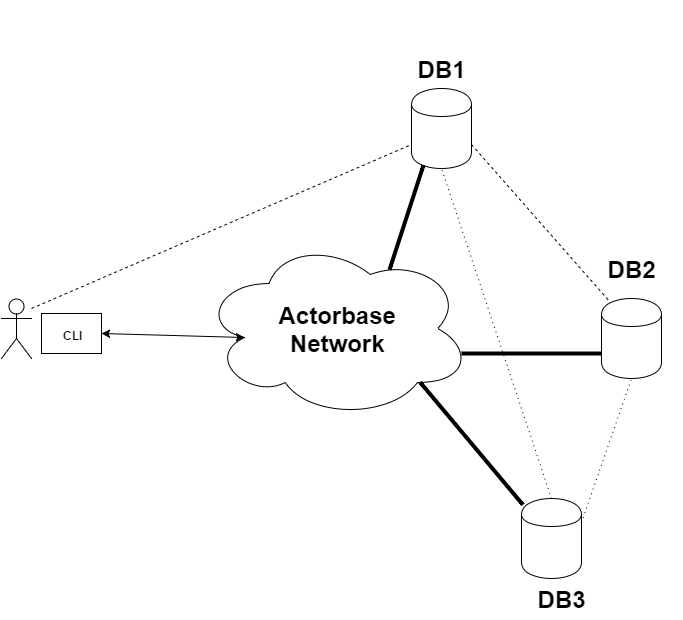
\includegraphics[width=0.7\textwidth,keepaspectratio]{UseCases/ActorbaseNetwork.png}
    \caption*{Actorbase: Visione generale semplificata rete Actorbase}
  \end{center}
\end{figure}

\subsection{UC1: Interazioni tramite CLI}

\begin{figure}[H]
  \begin{center}
    \includegraphics[width=0.7\textwidth,keepaspectratio]{UseCases/cli-generale.png}
    \caption*{Caso d'uso 1: Interazioni tramite CLI}
  \end{center}
\end{figure}
\textbf{Attori primari:} utente non autenticato, utente autenticato, utente amministratore\\
\textbf{Attore secondario:} Terminale\\
\textbf{Scopo e descrizione:} L'utente ha appena avviato la \gloss{CLI}, le operazioni che può eseguire sono:
\begin{itemize}
\item Nel caso sia un \textbf{utente non autenticato}:
  \begin{itemize}
  \item Effettuare il login
  \item Richiedere aiuto a livello generale o a livello di comando
  \end{itemize}
\item Nel caso sia un \textbf{utente autenticato} o un \textbf{utente amministratore}:
  \begin{itemize}
  \item Richiedere aiuto a livello generale o a livello di comando
  \item Effettuare operazioni sulle \gloss{collezioni}
  \item Effettuare operazioni sugli \gloss{item}
  \item Effettuare una ricerca su una o più \gloss{collezioni}
  \item Modificare la propria password
  \item Effettuare il logout
  \end{itemize}
\item Nel caso sia un \textbf{utente amministratore}:
  \begin{itemize}
  \item Effettuare operazioni di gestione utente
  \end{itemize}
\end{itemize}
\textbf{Precondizione:} il server è in ascolto\\
\textbf{Scenario principale utente non autenticato:}
\begin{itemize}
\item UC1.1\ -\ Login
\item UC1.2\ -\ Richiesta aiuto
  \begin{itemize}
  \item UC1.2.1\ -\ Aiuto generale
  \item UC1.2.2\ -\ Aiuto comando
  \end{itemize}
\end{itemize}
\textbf{Scenario principale utente autenticato o utente amministratore:}
\begin{itemize}
\item UC1.2\ -\ Richiesta aiuto
  \begin{itemize}
  \item UC1.2.1\ -\ Aiuto generale
  \item UC1.2.2\ -\ Aiuto comando
  \end{itemize}
\item UC1.3\ -\ Operazioni sulle collezioni
\item UC1.4\ -\ Operazioni sugli item
\item UC1.5\ -\ Ricerca su una o più collezioni
\item UC1.6\ -\ Modifica password
\item UC1.7\ -\ Logout
\end{itemize}
\textbf{Scenario principale utente amministratore:}
\begin{itemize}
\item UC1.8\ -\ Gestione utenti
\end{itemize}
\textbf{Estensioni:}
\begin{itemize}
\item Condizione: in UC1.1 l'utente inserisce una coppia username password non riconosciuta dal sistema:
  \begin{itemize}
  \item UC1.9\ -\ Visualizzazione errore credenziali errate
  \end{itemize}
\item Condizione: in UC1.6 l'utente inserisce una password attuale non corretta:
  \begin{itemize}
  \item UC1.10\ -\ Visualizzazione errore password attuale
  \end{itemize}
\item Condizione: in UC1.6 l'utente inserisce la password nuova che non rispetta i vincoli imposti dal sistema: %TODO scrivere questi vincoli da qualche parte
  \begin{itemize}
  \item UC1.11\ -\ Visualizzazione errore nuova password
  \end{itemize}
\item Condizione: in UC1.6 l'utente inserisce la nuova password per confermarne la modifica e risulta essere non corretta: %TODO vabene così?
  \begin{itemize}
  \item UC1.12\ -\ Visualizzazione errore conferma nuova password
  \end{itemize}
\end{itemize}
\textbf{Postcondizione:} Il sistema ha eseguito correttamente il comando inserito dall'utente.


\subsection{UC1.1: Login}

\begin{figure}[H]
  \begin{center}
    \includegraphics[width=0.7\textwidth,keepaspectratio]{UseCases/UC1_1.png}
    \caption*{Caso d'uso 1.1: Login}
  \end{center}
\end{figure}
\textbf{Attori primari:} Utente non autenticato\\
\textbf{Attori secondari:} Terminale\\
\textbf{Scopo e descrizione:}
L’utente ha appena avviato la \gloss{CLI}, risulta essere non autenticato e può effettuare il login diventando utente
autenticato.\\
\textbf{Precondizione:} Il server è in ascolto.\\
\textbf{Scenario principale:}
\begin{itemize}
\item UC1.1.1\ -\ Inserimento username;
\item UC1.1.2\ -\ Inserimento password.
\end{itemize}
\textbf{Estensioni:}
\begin{itemize}
\item Nel caso l'utente inserisca una coppia username-password non corrette:
  \begin{itemize}
  \item UC1.9 Visualizzazione Errore credenziali errate.
  \end{itemize}
\end{itemize}
\textbf{Postcondizioni:} L'utente ha acceduto al sistema con successo e risulta essere autenticato.

\subsubsection{UC1.1.1: Inserimento username}

\textbf{Attori primari:} Utente non autenticato\\
\textbf{Attori secondari:} Terminale\\
\textbf{Scopo e descrizione:}
L'utente ha appena avviato la \gloss{CLI}, risulta essere non autenticato e può inserire il proprio username per effettuare il login.\\
\textbf{Precondizioni:} Il server è in ascolto, l'utente ha inserito il comando per effettuare il login.
\textbf{Scenario principale:}
\begin{itemize}
\item L'utente può inserire il proprio username.
\end{itemize}
\textbf{Postcondizioni:} L'utente ha inserito il proprio username.

\subsubsection{UC1.1.2: Inserimento password}

\textbf{Attori primari:} Utente non autenticato\\
\textbf{Attori secondari:} Terminale\\
\textbf{Scopo e descrizione:}
L'utente ha appena avviato la \gloss{CLI}, risulta essere non autenticato e può inserire la propria password per effettuare il login.\\
\textbf{Precondizioni:} Il server è in ascolto, l'utente ha inserito il comando per effettuare il login e il suo username.
\textbf{Scenario principale:}
\begin{itemize}
\item L'utente può inserire la propria password.
\end{itemize}
\textbf{Postcondizioni:} L'utente ha inserito la propria password.

\subsection{UC1.2: Richiesta aiuto}

\textbf{Attori primari:} Utente non autenticato, Utente autenticato, Utente amministratore\\
\textbf{Attore secondario:} Terminale\\
\textbf{Scopo e descrizione:} L'utente intende richiedere aiuto sulla piattaforma o su un comando specifico.\\Nel caso di richiesta di aiuto generale diversi tipi di utente riceveranno la lista dei comandi da loro eseguibili\\
\textbf{Precondizione:} L'utente intende richiedere supporto.\\
\textbf{Scenario principale:}
\begin{itemize}
\item UC1.2.1\ -\ Aiuto generale;
\item UC1.2.2\ -\ Aiuto specifico.
\end{itemize}
\textbf{Postcondizioni:} Il sistema ha risposto producendo in output l'aiuto richiesto.

\subsection{UC1.2.1: Aiuto generale}

\textbf{Attore primario:} Utente non autenticato, Utente autenticato, Utente amministratore\\
\textbf{Attore secondario:} Terminale\\
\textbf{Scopo e descrizione:} L'utente intende richiedere aiuto generale sull'utilizzo del sistema \textbf{Actorbase}.\\
\textbf{Precondizione:} Il server è in ascolto.\\
\textbf{Scenario principale:}
\begin{itemize}
\item Inserimento comando di aiuto generale %TODO va tolto
\end{itemize}
\textbf{Postcondizioni:} Il sistema ha risposto visualizzando l'aiuto richiesto dall'utente in output.

\subsection{UC1.2.2: Aiuto specifico}

\textbf{Attore primario:} Utente non autenticato, Utente autenticato, Utente amministratore\\
\textbf{Attore secondario:} Terminale\\
\textbf{Scopo e descrizione:} L'utente intende richiedere aiuto su uno specifico comando del sistema \textbf{Actorbase}.\\
\textbf{Precondizione:} Il server è in ascolto.\\
\textbf{Scenario principale:}
\begin{itemize}
\item UC1.2.2.1\ -\ Inserimento nome comando.
\end{itemize}
\textbf{Postcondizioni:} Il sistema ha risposto visualizzando l'aiuto richiesto dall'utente in output.

\subsubsection{UC1.2.2.1: Inserimento nome comando}

\textbf{Attore primario:} Utente non autenticato, Utente autenticato, Utente amministratore\\
\textbf{Attore secondario:} Terminale\\
\textbf{Scopo e descrizione:} L'utente intende richiedere aiuto specifico sull'utilizzo di un preciso comando del sistema.\\
\textbf{Precondizione:} Il server è in ascolto e l'utente ha inserito il comando di aiuto specifico.\\
\textbf{Scenario principale:}
\begin{itemize}
\item Inserimento nome comando %TODO va messo sto caso d'uso? sto sclerando e sono solo le 11.39
\end{itemize}
\textbf{Postcondizioni:} Il sistema ha risposto visualizzando l'aiuto richiesto dall'utente in output.

\subsection{UC1.3: Operazioni sulle collezioni}

\begin{figure}[H]
  \begin{center}
    \includegraphics[width=0.7\textwidth,keepaspectratio]{UseCases/UC1_3.png}
    \caption*{Caso d'uso 1.3: Operazioni sulle \gloss{collezioni}}
  \end{center}
\end{figure}
\textbf{Attore primario:} Utente autenticato\\
\textbf{Attore secondario:} Terminale\\
\textbf{Scopo e descrizione:} L'utente è autenticato e desidera effettuare delle operazioni sulle \gloss{collezioni}. Le operazioni previste sono:
creazione di una nuova \gloss{collezione}, visualizzazione della lista delle \gloss{collezioni} esistenti, cancellazione di \gloss{collezioni} esistenti, modifica del nome di \gloss{collezioni} esistenti e
aggiunta o rimozione collaboratori a \gloss{collezione} esistente.\\
\textbf{Precodizione:} L'utente intende effettuare operazioni su \gloss{collezioni}.\\
\textbf{Scenario principale:}
\begin{itemize}
\item UC1.3.1\ -\ Creazione \gloss{collezione};
\item UC1.3.2\ -\ Visualizzazione della lista delle \gloss{collezioni};
\item UC1.3.3\ -\ Cancellazione \gloss{collezione};
\item UC1.3.4\ -\ Modifica nome \gloss{collezione};
\item UC1.3.5\ -\ Aggiunta \gloss{collaboratore};
\item UC1.3.6\ -\ Rimozione \gloss{collaboratore};
\item UC1.3.7\ -\ Esportazione di una o più collezioni su file.
\end{itemize}
\textbf{Estensioni:}
\begin{itemize}
\item Nel caso in cui nelle procedure di creazione collezione o modifica nome collezione, l'utente inserisca il nome di una collezione già censita all'iterno del sistema:
  \begin{itemize}
  \item UC1.3.10\ -\ Visualizzazione errore \gloss{collezione} già esistente.
  \end{itemize}
\item Nel caso in cui nelle procedure di modifica, cancellazione collezione, aggiunta collaboratore a collezione o rimozione collaboratore a collezione, l'utente inserisca il nome di una collezione non censita all'interno del sistema:
  \begin{itemize}
  \item UC1.3.8\ -\ Visualizzazione errore collezione inesistente.
  \end{itemize}
\item Nel caso in cui nelle procedure di aggiunta o rimozione collaboratore a collezione l'utente inserisca uno username non censito all'interno del sistema:
  \begin{itemize}
  \item UC1.3.9\ -\ Visualizzazione errore username inesistente.
  \end{itemize}
\end{itemize}
\textbf{Postcondizioni:} L'operazione richiesta è stata eseguita con successo.

\subsection{UC1.3.1: Creazione collezione}

\textbf{Attore primario:} Utente autenticato\\
\textbf{Attore secondario:} Terminale\\
\textbf{Scopo e descrizione:} L'utente richiede la creazione di una \gloss{collezione} all'interno del \gloss{database}, deve inserire il nome della nuova \gloss{collezione}.\\
\textbf{Precodizione:} Il \gloss{database} è pronto a ricevere comandi e l'utente intende creare una \gloss{collezione}.\\
\textbf{Scenario principale:}
\begin{itemize}
\item L'utente può inserire il nome \gloss{collezione} % TODO qua bisogna mettere il sotto caso d'uso utente inserisce nome collezione da creare? credo di si
\end{itemize}
\textbf{Postcondizioni:} La \gloss{collezione} è stata creata.

\subsection{UC1.3.2: Visualizzazione della lista delle collezioni}

\textbf{Attore primario:} Utente autenticato\\
\textbf{Attore secondario:} Terminale\\
\textbf{Scopo e descrizione:} L'utente intende elencare tutte le \gloss{collezioni} all'interno di \textbf{Actorbase} secondo la propria \gloss{visibilità}.\\
\textbf{Precodizione:} Il \gloss{database} è pronto a ricevere comandi e l'utente intende elencare le \gloss{collezioni} al suo interno.\\
\textbf{Scenario principale:}
\begin{itemize}
\item Inserimento nome collezione.
\end{itemize}
\textbf{Postcondizioni:} Il \gloss{database} restituisce la lista delle \gloss{collezioni} esistenti secondo la \gloss{visibilità} dell'utente, per ogni collezione viene visualizzato il nome della collezione stessa.

\subsection{UC1.3.3: Modifica nome collezione}

\begin{figure}[H]
  \begin{center}
    \includegraphics[width=0.7\textwidth,keepaspectratio]{UseCases/UC1_3_3.png}
    \caption*{Caso d'uso 1.3.3: Login}
  \end{center}
\end{figure}
\textbf{Attore primario:} Utente autenticato\\
\textbf{Attore secondario:} Terminale\\
\textbf{Scopo e descrizione:} L’utente intende modificare il nome di una \gloss{collezione} presente nel \gloss{database}.\\
\textbf{Precodizione:} Il server è in ascolto e l’utente intende modificare il nome di una \gloss{collezione}.\\
\textbf{Scenario principale:}
\begin{itemize}
\item UC1.3.3.1\ -\ Inserimento nome \gloss{collezione};
\item UC1.3.3.2\ -\ Inserimento nuovo nome \gloss{collezione}.
\end{itemize}
\textbf{Estensioni:}
\begin{itemize}
\item Nel caso in cui l'utente inserisca come nuovo nome per la collezione da modificare, un nome di una collezione già esistente all'interno del sistema:
  \begin{itemize}
  \item UC1.3.10\ -\ Visualizzazione errore collezione già esistente.
  \end{itemize}
\item Nel caso in cui l'utente inserisca come nome della collezione da modificare, un nome di una collezione inesistente all'interno del sistema:
  \begin{itemize}
  \item UC1.3.8\ -\ Visualizzazione errore collezione inesistente.
  \end{itemize}
\end{itemize}
\textbf{Postcondizioni:} Il nome della \gloss{collezione} è stato modificato correttamente.

\subsubsection{UC1.3.3.1: Inserimento nome collezione}

\textbf{Attore primario:} Utente autenticato\\
\textbf{Attore secondario:} Terminale\\
\textbf{Scopo e descrizione:} L'utente intende modificare il nome di un \gloss{collezione} presente nel \gloss{database}, deve inserire il nome della collezione da modificare.\\
\textbf{Precondzione:} Il server è in ascolto e l'utente intende modificare il nome di una \gloss{collezione}, deve inserire il nome della collezione da modificare.\\
\textbf{Scenario principale:}
\begin{itemize}
\item L'utente può inserire il nome della collezione da modificare.
\end{itemize}
\textbf{Postcondizioni:} Il nome della \gloss{collezione} da modificare è stato inserito

\subsubsection{UC1.3.3.2: Inserimento nuovo nome collezione}

\textbf{Attore primario:} Utente autenticato\\
\textbf{Attore secondario:} Terminale\\
\textbf{Scopo e descrizione:} L'utente intende modificare il nome di un \gloss{collezione} presente nel \gloss{database}, deve inserire il nuovo nome della collezione da modificare.\\
\textbf{Precondzione:} Il server è in ascolto e l'utente intende modificare il nome di una \gloss{collezione}, deve inserire il nuovo nome della collezione da modificare.\\
\textbf{Scenario principale:}
\begin{itemize}
\item L'utente può inserire il nuovo nome della collezione da modificare.
\end{itemize}
\textbf{Postcondizioni:} Il nuovo nome della \gloss{collezione} da modificare è stato inserito

\subsection{UC1.3.4: Cancellazione collezione}

\textbf{Attore primario:} Utente autenticato\\
\textbf{Attore secondario:} Terminale\\
\textbf{Scopo e descrizione:} L’utente intende cancellare una \gloss{collezione} presente nel \gloss{database}.\\
\textbf{Precodizione:} Il server è in ascolto e l’utente intende cancellare una \gloss{collezione}.\\
\textbf{Scenario principale:}
\begin{itemize}
\item UC1.3.4.1\ -\ Inserimento nome \gloss{collezione}.
\end{itemize}
\textbf{Estensioni:}
\begin{itemize}
\item Nel caso in cui l'utente inserisca il nome di una collezione da cancellare inesistente:
  \begin{itemize}
  \item UC1.3.8\ -\ Visualizzazione errore \gloss{collezione} inesistente;
  \end{itemize}
\end{itemize}
\textbf{Postcondizioni:} La \gloss{collezione} è stato cancellata correttamente.

\subsubsection{UC1.3.4.1: Inserimento nome collezione}

\textbf{Attore primario:} Utente autenticato\\
\textbf{Attore secondario:} Terminale\\
\textbf{Scopo e descrizione:} L'utente intende cancellare il nome di un \gloss{collezione} presente nel \gloss{database}, deve inserire il nome della collezione da cancellare.\\
\textbf{Precondzione:} Il server è in ascolto e l'utente intende cancellare il nome di una \gloss{collezione}, deve inserire il nome della collezione da cancellare.\\
\textbf{Scenario principale:}
\begin{itemize}
\item L'utente può inserire il nome della collezione da cancellare.
\end{itemize}
\textbf{Postcondizioni:} Il nome della \gloss{collezione} da cancellare è stato inserito

\subsection{UC1.3.5: Aggiunta di un collaboratore a collezione}

\begin{figure}[H]
  \begin{center}
    \includegraphics[width=0.7\textwidth,keepaspectratio]{UseCases/UC1_3_5.png}
    \caption*{Caso d'uso 1.3.5: aggiunta di un collaboratore a collezione}
  \end{center}
\end{figure}
\textbf{Attore primario:} Utente autenticato\\
\textbf{Attore secondario:} Terminale\\
\textbf{Scopo e descrizione:} L'utente intende aggiungere un \gloss{collaboratore} ad una \gloss{collezione} di sua proprietà. Deve inserire il nome della \gloss{collezione} e lo username dell'utente da aggiungere.\\
\textbf{Precondizione:} Il \gloss{database} è pronto a ricevere comandi e l'utente intende aggiungere un \gloss{collaboratore} ad una \gloss{collezione} di sua proprietà.\\
\textbf{Scenario principale:}
\begin{itemize}
\item UC1.3.5.1\ -\ Inserimento nome \gloss{collezione};
\item UC1.3.5.2\ -\ Inserimento username \gloss{collaboratore}.
\end{itemize}
\textbf{Postcondizioni:} L'utente designato per la collaborazione è stato aggiunto tra i \gloss{collaboratori} della \gloss{collezione} scelta.

\subsubsection{UC1.3.5.1: Inserimento nome collezione}

\textbf{Attore primario:} Utente autenticato\\
\textbf{Attore secondario:} Terminale\\
\textbf{Scopo e descrizione:} L'utente intende aggiungere un \gloss{collaboratore} ad una \gloss{collezione} di sua proprietà; deve inserire il nome della collezione in questione.\\
\textbf{Precondizione:} Il server è in ascolto e l'utente ha inserito il comando per l'aggiunta di un \gloss{collaboratore} ad una \gloss{collezione}.
\textbf{Scenario principale:}
\begin{itemize}
\item L'utente può inserire il nome della \gloss{collezione}.
\end{itemize}
\textbf{Postcondizioni:} Il nome della \gloss{collezione} designata all'aggiunta di un \gloss{collaboratore} è stato inserito correttamente.

\subsubsection{UC1.3.5.2: Inserimento username collaboratore}

\textbf{Attore primario:} Utente autenticato\\
\textbf{Attore secondario:} Terminale\\
\textbf{Scopo e descrizione:} L'utente intende aggiungere un \gloss{collaboratore} ad una \gloss{collezione} di sua proprietà; deve inserire lo username del collaboratore da aggiugere.\\
\textbf{Precondizione:} Il server è in ascolto, l'utente ha inserito il comando per l'aggiunta di un \gloss{collaboratore} ad una \gloss{collezione} e ha inserito il nome della \gloss{collezione}.\\
\textbf{Scenario principale:}
\begin{itemize}
\item L'utente può inserire il nome del \gloss{collaboratore}.
\end{itemize}
\textbf{Postcondizioni:} Il nome del collaboratore designato all'aggiunta ad una collezione è stato inserito correttamente.

\subsection{UC1.3.6: Rimozione di un collaboratore da collezione}
\begin{figure}[H]
  \begin{center}
    \includegraphics[width=0.7\textwidth,keepaspectratio]{UseCases/UC1_3_6.png}
    \caption*{Caso d'uso 1.3.6: rimozione di un collaboratore da una collezione}
  \end{center}
\end{figure}
\textbf{Attore primario:} Utente autenticato\\
\textbf{Scopo e descrizione:} L'utente intende rimuovere un \gloss{collaboratore} da una \gloss{collezione} di sua proprietà. Deve inserire il nome della \gloss{collezione} e lo username del \gloss{collaboratore} da rimuovere.\\
\textbf{Precondizione:} Il \gloss{database} è pronto a ricevere comandi e l'utente intende rimuovere un \gloss{collaboratore} da una \gloss{collezione} di sua proprietà.\\
\textbf{Scenario principale:}
\begin{itemize}
\item UC1.3.6.1\ -\ Inserimento nome \gloss{collezione};
\item UC1.3.6.2\ -\ Inserimento username \gloss{collaboratore}.
\end{itemize}
\textbf{Postcondizione:} L'utente designato per la rimozione dai \gloss{collaboratori} è stato rimosso dalla \gloss{collezione} scelta.

\subsubsection{UC1.3.6.1: Inserimento nome collezione}

\textbf{Attore primario:} Utente autenticato\\
\textbf{Attore secondario:} Terminale\\
\textbf{Scopo e descrizione:} L'utente intende aggiungere un \gloss{collaboratore} ad una \gloss{collezione} di sua proprietà; deve inserire il nome della collezione in questione.\\
\textbf{Precondizione:} Il server è in ascolto e l'utente ha inserito il comando per la rimozione di un collaboratore da una collezione.
\textbf{Scenario principale:}
\begin{itemize}
\item L'utente può inserire il nome della collezione.
\end{itemize}
\textbf{Postcondizioni:} Il nome della collezione designata all'aggiunta di un collaboratore è stato inserito correttamente.

\subsubsection{UC1.3.6.2: Inserimento username collaboratore}

\textbf{Attore primario:} Utente autenticato\\
\textbf{Attore secondario:} Terminale\\
\textbf{Scopo e descrizione:} L'utente intende aggiungere un \gloss{collaboratore} ad una \gloss{collezione} di sua proprietà; deve inserire lo username del collaboratore da aggiugere.\\
\textbf{Precondizione:} Il server è in ascolto, l'utente ha inserito il comando per la rimozione di un collaboratore da una collezione e ha inserito il nome della \gloss{collezione}.\\
\textbf{Scenario principale:}
\begin{itemize}
\item L'utente può inserire il nome del collaboratore.
\end{itemize}
\textbf{Postcondizioni:} Il nome del collaboratore designato all'aggiunta ad una collezione è stato inserito correttamente.

\subsection{UC1.3.7: Esportazione su file}

\textbf{Attore primario:} Utente autenticato\\
\textbf{Attore secondario:} Terminale\\
\textbf{Scopo e descrizione:} L'utente intende esportare su file il contenuto di una o più collezioni\\
\textbf{Precondizione:} Il server è in ascolto e l'utente intende esportare il contenuto di una o più collezioni su file.
\textbf{Scenario principale:}
\begin{itemize}
\item L'utente può inserire la lista di collezioni da esportare. %TODO bisogna emttere il sotto caso d'uso inserire lista collezioni?
\end{itemize}
\textbf{Postcondizione:} Il contenuto delle collezioni selezionate è stato esportato su file.

\subsection{UC1.3.8: Visualizzazione errore username inesistente}

\textbf{Attori primari:} Utente autenticato\\
\textbf{Attori secondari:} Terminale\\
\textbf{Scopo e descrizione:}
L'utente ha inserito un comando tra:
\begin{itemize}
\item UC1.3.5\ -\ Aggiunta collaboratore a collezione
\item UC1.3.6\ -\ Rimozione collaboratore da collezione
\end{itemize}
e i parametri per la sua esecuzione tra cui lo username che risulta essere non già censito all'interno del sistema.\\
\textbf{Precondizioni:} Il server è in ascolto, l'utente ha inserito il %finire tutti i casi di errore qua sotto
comando per la modifica password, ha inserito i parametri necessari (password attuale, nuova password e password di conferma) e intende modificare la propria password. Il sistema non riconosce la password di conferma inserita.\\
\textbf{Scenario principale:}
\begin{itemize}
\item Viene visualizzato un messaggio di errore esplicativo.
\end{itemize}
\textbf{Postcondizioni:} La modifica password fallisce, la password dell'utente resta quella di prima.

\subsection{UC1.3.9: Visualizzazione errore collezione inesistente}

\textbf{Attori primari:} Utente autenticato\\
\textbf{Attori secondari:} Terminale\\
\textbf{Scopo e descrizione:}
L'utente ha inserito il comando per la modifica password, ha inserito i parametri necessari (password attuale, nuova password e password di conferma) per modificare la propria password.\\
\textbf{Precondizioni:} Il server è in ascolto, l'utente ha inserito il comando per la modifica password, ha inserito i parametri necessari (password attuale, nuova password e password di conferma) e intende modificare la propria password. Il sistema non riconosce la password di conferma inserita.\\
\textbf{Scenario principale:}
\begin{itemize}
\item Viene visualizzato un messaggio di errore esplicativo.
\end{itemize}
\textbf{Postcondizioni:} La modifica password fallisce, la password dell'utente resta quella di prima.

\subsection{UC1.3.10: Visualizzazione errore collezione già esistente}

\textbf{Attori primari:} Utente autenticato\\
\textbf{Attori secondari:} Terminale\\
\textbf{Scopo e descrizione:}
L'utente ha inserito il comando per la modifica password, ha inserito i parametri necessari (password attuale, nuova password e password di conferma) per modificare la propria password.\\
\textbf{Precondizioni:} Il server è in ascolto, l'utente ha inserito il comando per la modifica password, ha inserito i parametri necessari (password attuale, nuova password e password di conferma) e intende modificare la propria password. Il sistema non riconosce la password di conferma inserita.\\
\textbf{Scenario principale:}
\begin{itemize}
\item Viene visualizzato un messaggio di errore esplicativo.
\end{itemize}
\textbf{Postcondizioni:} La modifica password fallisce, la password dell'utente resta quella di prima.

\subsection{UC1.4: Operazioni sugli item}
\begin{figure}[H]
  \begin{center}
    \includegraphics[width=0.7\textwidth,keepaspectratio]{UseCases/UC1_4.png}
    \caption*{Caso d'uso 1.4: Operazioni sugli \gloss{item}}
  \end{center}
\end{figure}
\textbf{Attore primario:} Utente autenticato\\
\textbf{Atttore secondario:} Terminale\\
\textbf{Scopo e descrizione:} L'utente intende effettuare operazioni sugli \gloss{item} di una \gloss{collezione} esistente. Le operazioni previste sono:
inserimento e cancellazione.\\
\textbf{Precondizione:} Il \gloss{database} è pronto a ricevere comandi e l'utente intende effettuare operazioni di inserimento o cancellazione su una \gloss{collezione} esistente.\\
\textbf{Scenario principale:}
\begin{itemize}
\item UC1.4.1\ -\ Inserimento nuovo \gloss{item};
  \begin{itemize}
  \item UC1.4.1.1\ -\ Inserimento \gloss{item} manuale;
  \item UC1.4.1.2\ -\ Inserimento \gloss{item} item da file.
  \end{itemize}
\item UC1.4.2\ -\ Cancellazione \gloss{item}.
\end{itemize}
\textbf{Estensioni:}
\begin{itemize}
\item Nel caso in cui la \gloss{collezione} su cui effettuare cancellazione non sia presente:
  \begin{itemize}
  \item UC1.4.5\ -\ Visualizzazione errore collezione inesistente.
  \end{itemize}
\item Nel caso in cui la chiave dell'item da inserire sia già presente:
  \begin{itemize}
  \item UC1.4.4\ -\ Visualizzazione errore chiave già esistente.
  \end{itemize}
\item Nel caso in cui la collezione su cui effettuare l'inserimento sia inesistente:
  \begin{itemize}
  \item UC1.4.6\ -\ Creazione nuova collezione.
  \end{itemize}
\item Nel caso in cui il file che contiene gli item da inserire non sia presente nel path inserito:
  \begin{itemize}
  \item UC1.4.3\ -\ Visualizzazione errore file inesistente.
  \end{itemize}
\end{itemize}
\textbf{Postcondizione:} L'operazione richiesta è stata effettuata correttamente.

\subsection{UC1.4.1: Inserimento item}

\textbf{Attore primario:} Utente autenticato\\
\textbf{Attore secondario:} Terminale\\
\textbf{Scopo e descrizione:} L'utente intende inserire un nuovo \gloss{item} all'interno di una \gloss{collezione} esistente. Deve selezionare la \gloss{collezione} e inserire i parametri di definizione dell'\gloss{item}. Questi sono la chiave, il valore associato e il \gloss{flag} di sovrascrittura. Può scegliere di inserire mediante due modalità distinte:
\begin{itemize}
\item Manuale;
\item Da file.
\end{itemize}
\textbf{Precondizione:} Il \gloss{database} è pronto a ricevere comandi e l'utente intende effettuare un inserimento di un nuovo \gloss{item}.\\
\textbf{Scenario principale:}
\begin{itemize}
\item UC1.4.1.1\ -\ Inserimento item manuale;
\item UC1.4.1.2\ -\ Inserimento item da file.
\end{itemize}
\textbf{Postcondizioni:} L'operazione di inserimento richiesta è stata effettuata correttamente.

\subsection{UC1.4.1.1: Inserimento item manuale}
\begin{figure}[H]
  \begin{center}
    \includegraphics[width=0.7\textwidth,keepaspectratio]{UseCases/UC1_4_1_1.png}
    \caption*{Caso d'uso 1.4.1.1: Inserimento item manuale}
  \end{center}
\end{figure}
\textbf{Attore primario:} Utente autenticato\\
\textbf{Attore secondario} Terminale\\
\textbf{Scopo e descrizione:} L'utente intende inserire manualmente un nuovo \gloss{item} all'interno di una \gloss{collezione} esistente. Deve selezionare la \gloss{collezione} e inserire i parametri di definizione dell'\gloss{item}. Questi sono la chiave, il valore associato e il \gloss{flag} di sovrascrittura.\\
\textbf{Precondizione:} Il server è in ascolto e l'utente intende inserire un nuovo item in modalità manuale.\\
\textbf{Scenario principale:}
\begin{itemize}
\item UC1.4.1.1.1\ -\ Inserimento nome collezione;
\item UC1.4.1.1.2\ -\ Inserimento chiave;
\item UC1.4.1.1.3\ -\ Inserimento valore;
\item UC1.4.1.1.4\ -\ Inserimento flag sovrascrittura.
\end{itemize}
\textbf{Estensioni:}
\begin{itemize}
\item Nel caso in cui l'utente inserisca un item con \gloss{flag} di sovrascrittura attivo contenente una chiave già esistente all'interno del sistema:
  \begin{itemize}
  \item UC1.4.4\ -\ Visualizzazione errore chiave già esistente.
  \end{itemize}
\end{itemize}
\textbf{Postcondizioni:} L'item è stato inserito con successo

\subsubsection{UC1.4.1.1.1: Inserimento nome collezione}

\textbf{Attore primario:} Utente autenticato\\
\textbf{Attore secondario:} Terminale\\
\textbf{Scopo e descrizione:} L'utente intende inserire manualmente un nuovo \gloss{item} all'interno di una \gloss{collezione} esistente. Deve inserire il nome della collezione.\\
\textbf{Precondizione:} Il server è in ascolto e l'utente ha inserito il comando per l'inserimento item manuale.\\
\textbf{Scenario principale:}
\begin{itemize}
\item L'utente può inserire il nome della collezione su cui effettuare l'inserimento.
\end{itemize}
\textbf{Estensioni:}
\begin{itemize}
\item Nel caso in cui l'utente inserisca il nome di una collezione non esistente all'interno del sistema:
  \begin{itemize}
  \item UC4.6\ -\ Creazione nuova collezione. %TODO non so se sia proprio giusto
  \end{itemize}
\end{itemize}
\textbf{Postcondizione:} Il nome della collezione è stato inserito correttamente.

\subsubsection{UC1.4.1.1.2: Inserimento chiave}

\textbf{Attore primario:} Utente autenticato\\
\textbf{Attore secondario:} Terminale\\
\textbf{Scopo e descrizione:} L'utente intende inserire manualmente un nuovo \gloss{item} all'interno di una \gloss{collezione} esistente. Deve inserire la chiave dell'item.\\
\textbf{Precondizione:} Il server è in ascolto, l'utente ha inserito il comando per l'inserimento item manuale e ha inserito il nome della collezione.\\
\textbf{Scenario principale:}
\begin{itemize}
\item L'utente può inserire la chiave associata all'item.
\end{itemize}
\textbf{Estensioni:}
\begin{itemize}
\item Nel caso in cui l'utente inserisca un item con \gloss{flag} di sovrascrittura attivo associato ad una chiave già presente all'interno del sistema:
  \begin{itemize}
  \item UC1.4.4\ -\ Visualizzazione errore chiave già esistente
  \end{itemize}
\end{itemize}
\textbf{Postcondizioni:} La chiave è stata inserita correttamente.

\subsubsection{UC1.4.1.1.3: Inserimento valore}

\textbf{Attore primario:} Utente autenticato\\
\textbf{Attore secondario:} Terminale\\
\textbf{Scopo e descrizione:} L'utente intende inserire manualmente un nuovo \gloss{item} all'interno di una \gloss{collezione} esistente. Deve inserire il valore associato alla chiave dell'item.\\
\textbf{Precondizione:} Il server è in ascolto, l'utente ha inserito il comando per l'inserimento item manuale, ha inserito il nome della collezione e ha inserito la chiave.\\
\textbf{Scenario principale:}
\begin{itemize}
\item L'utente può inserire il valore associato alla chiave dell'item.
\end{itemize}
\textbf{Postcondizioni:} Il valore è stato inserito correttamente.

\subsubsection{UC1.4.1.1.4: Inserimento flag sovrascrittura}

\textbf{Attore primario:} Utente autenticato\\
\textbf{Attore secondario:} Terminale\\
\textbf{Scopo e descrizione:} L'utente intende inserire manualmente un nuovo \gloss{item} all'interno di una \gloss{collezione} esistente. Deve inserire il \gloss{flag} di sovrascrittura item.\\
\textbf{Precondizione:} Il server è in ascolto, l'utente ha inserito il comando per l'inserimento item manuale, ha inserito il nome della collezione, ha inserito la chiave e il valore dell'\gloss{item}.\\
\textbf{Scenario principale:}
\begin{itemize}
\item L'utente può inserire il \gloss{flag} di sovrascrittura item. %TODO il flag può fare errore... lo inglobiamo negli errori di battitura?
\end{itemize}
\textbf{Postcondizioni:} Il \gloss{flag} è stato inserito correttamente.

\subsection{UC1.4.1.2: Inserimento item da file}

\begin{figure}[H]
  \begin{center}
    \includegraphics[width=0.7\textwidth,keepaspectratio]{UseCases/UC1_4_1_2.png}
    \caption*{Caso d'uso 1.4.1.2: Inserimento \gloss{item} da file}
  \end{center}
\end{figure}
\textbf{Attore primario:} Utente\\
\textbf{Attore secondario:} Terminale\\
\textbf{Scopo e descrizione:} L'utente intende inserire nuovi \gloss{item} da file. Deve inserire il \gloss{path} del file su filesystem.\\
\textbf{Precondizione:} Il server è in ascolto e l'utente intende inserire nuovi \gloss{item} da file.\\
\textbf{Scenario principale:}
\begin{itemize}
\item L'utente può inserire \gloss{path} del file.
\end{itemize}
\textbf{Estensioni:}
\begin{itemize}
\item Nel caso in cui il file non esista nel filesystem:
  \begin{itemize}
  \item UC1.4.3\ -\ Visualizzazione errore file inesistente.
  \end{itemize}
  % TODO se il file è "costruito male" credo sia un altro errore da aggiungere qua
\end{itemize}
\textbf{Postcondizioni:} Gli item scritti all'interno del file inserito sono stati inseriti con successo all'interno del sistema.%TODO vaben così? %Il \gloss{path} è stato inserito correttamente.

\subsubsection{UC1.4.1.2.1: Inserimento path file}

\textbf{Attore primario:} Utente autenticato\\
\textbf{Attore secondario:} Terminale\\
\textbf{Scopo e descrizione:} L'utente intende inserire nuovi \gloss{item} da file. Deve inserire il \gloss{path} del file su filesystem.\\
\textbf{Precondizione:} Il server è in ascolto e l'utente ha inserito il comando per l'inserimento di \gloss{item} da file.\\
\textbf{Scenario principale:}
\begin{itemize}
\item L'utente può inserire il \gloss{path} del file.
\end{itemize}
\textbf{Postcondizioni:} Il \gloss{path} è stato inserito correttamente.

\subsection{UC1.4.2: Cancellazione item}

\begin{figure}[H]
  \begin{center}
    \includegraphics[width=0.7\textwidth,keepaspectratio]{UseCases/UC1_4_2.png}
    \caption*{Caso d'uso 1.4.2: Cancellazione \gloss{item}}
  \end{center}
\end{figure}
\textbf{Attore primario:} Utente autenticato\\
\textbf{Attore secondario:} Terminale\\
\textbf{Scopo e descrizione:} L'utente intende cancellare un item da una collezione.\\
\textbf{Precondizioni:} Il server è in ascolto e l'utente intende cancellare un item.\\
\textbf{Scenario principale:}
\begin{itemize}
\item UC1.4.2.1\ -\ Inserimento nome \gloss{collezione};
\item UC1.4.2.2\ -\ Inserimento chiave \gloss{item}.
\end{itemize}
\textbf{Estensioni:}
\begin{itemize}
\item Nel caso in cui l'utente inserisca il nome di una \gloss{collezione} inesistente:
  \begin{itemize}
  \item UC1.4.5\ -\ Visualizzazione errore collezione inesistente.
  \end{itemize}
\end{itemize}
\textbf{Postcondizioni:} L'\gloss{item} è stato cancellato correttamente.

\subsection{UC1.4.2.1: Inserimento nome collezione}

\textbf{Attore primario:} Utente autenticato\\
\textbf{Attore secondario:} Terminale\\
\textbf{Scopo e descrizione:} L'utente intende cancellare un \gloss{item} all'interno di una \gloss{collezione} esistente. Deve inserire il nome della collezione.\\
\textbf{Precondizione:} Il server è in ascolto e l'utente ha inserito il comando di cancellazione item.\\
\textbf{Scenario principale:}
\begin{itemize}
\item L'utente può inserire il nome della collezione su cui effettuare la cancellazione.
\end{itemize}
\textbf{Postcondizione:} Il nome della collezione è stato inserito correttamente.

\subsection{UC1.4.2.2: Inserimento chiave item}

\textbf{Attore primario:} Utente autenticato\\
\textbf{Attore secondario:} Terminale\\
\textbf{Scopo e descrizione:} L'utente intende cancellare un \gloss{item} all'interno di una \gloss{collezione} esistente. Deve inserire la chiave dell'item.\\
\textbf{Precondizione:} Il server è in ascolto, l'utente ha inserito il comando di cancellazione item e ha inserito il nome della collezione.\\
\textbf{Scenario principale:}
\begin{itemize}
\item L'utente può inserire la chiave dell'item da eliminare.
\end{itemize}
\textbf{Postcondizioni:} La chiave è stata inserita correttamente.

\subsection{UC1.5: Ricerca}

\textbf{Attore primario:} Utente autenticato\\
\textbf{Attore secondario:} Terminale\\
\textbf{Scopo e descrizione:} L'utente intende effettuare una ricerca di \gloss{item} all'interno del sistema; può decidere di effettuare la ricerca su una lista di collezioni eventualmente vuota, in tal caso la
ricerca verrà estesa a tutto il sistema entro i limiti imposti dal grado di visibilità (vedi~\ref{sec:visibilità}) dell'utente.\\
In caso di inserimento di nome \gloss{collezione} inesistente, o in caso di risultati di ricerca nulli, il sistema riporterà una lista risultata vuota.\\ % TODO: stesso per chiavi?
\textbf{Precondizione:} Il server è in ascolto, l'utente intende effettuare una ricerca di \gloss{item} all'interno del sistema.\\
\textbf{Scenario principale:}
\begin{itemize}
\item UC1.5.1\ -\ Inserimento lista collezioni;
\item UC1.5.2\ -\ Inserimento chiave di ricerca.
\end{itemize}
\textbf{Postcondizioni:} Il sistema ha riportato la lista dei risultati di ricerca.

\subsection{UC1.5.1: Inserimento lista collezioni}

\textbf{Attore primario:} Utente autenticato\\
\textbf{Attore secondario:} Terminale\\
\textbf{Scopo e descrizione:} L'utente intende effettuare una ricerca di \gloss{item} all'interno del sistema; deve inserire la lista delle collezioni su cui effettuare tale ricerca. In caso di lista di ricerca vuota
la funzione di ricerca verrà estesa a tutto il sistema entro i limit imposti dal grado di visibilità (vedi~\ref{sec:visibilità}) dell'utente.\\
In caso di inserimento di nome \gloss{collezione} inesistente, o in caso di risultati di ricerca nulli, il sistema riporterà una lista risultata vuota.\\ % TODO: stesso per chiavi?
\textbf{Precondizione:} Il server è in ascolto, l'utente intende effettuare una ricerca di \gloss{item} all'interno del  sistema.\\
\textbf{Scenario principale:}
\begin{itemize}
\item Inserimento lista collezioni.
\end{itemize}
\textbf{Postcondizioni:} La lista di collezioni su cui effettuare la ricerca è stata inserita correttamente.

\subsection{UC1.5.2: Inserimento chiave di ricerca}

\textbf{Attore primario:} Utente autenticato\\
\textbf{Attore secondario:} Terminale\\
\textbf{Scopo e descrizione:} L'utente intende effettuare una ricerca di \gloss{item} all'interno del sistema; deve inserire la chiave di cui effettuare tale ricerca.\\
In caso di inserimento di nome \gloss{collezione} inesistente, o in caso di risultati di ricerca nulli, il sistema riporterà una lista risultata vuota.\\ % TODO: stesso per chiavi?
\textbf{Precondizione:} Il server è in ascolto, l'utente intende effettuare una ricerca di \gloss{item} all'interno del  sistema.\\
\textbf{Scenario principale:}
\begin{itemize}
\item Inserimento chiave di ricerca
\end{itemize}
\textbf{Postcondizioni:} La chiave da ricerca all'interno del sistema è stata inserita correttamente.

\subsection{UC1.6: Modifica password}
% TODO: dialogo
\begin{figure}[H]
  \begin{center}
    \includegraphics[width=0.7\textwidth,keepaspectratio]{UseCases/UC1_6.png}
    \caption*{Caso d'uso 1.6: Modifica password}
  \end{center}
\end{figure}
\textbf{Attori primari:} Utente autenticato\\
\textbf{Attori secondari:} Terminale\\
\textbf{Scopo e descrizione:} L'utente intende modificare la propria password, deve inserire la propria password attuale, inserire poi la nuova password e confermarla.\\
\textbf{Precondizione:} Il server è in ascolto.
\textbf{Scenario principale:}
\begin{itemize}
\item UC1.6.1\ -\ Inserimento password attuale;
\item UC1.6.2\ -\ Inserimento nuova password;
\item UC1.6.3\ -\ Conferma password.
\end{itemize}
\textbf{Estensioni:} %TODO controllare ste estensioni
\begin{itemize}
\item In UC1.6.1\ -\ l'utente inserisce una password attuale non corretta:
  \begin{itemize}
  \item UC1.6.4\ -\ Visualizzazione errore password attuale
  \end{itemize}
\item In UC1.6.2\ -\ l'utente inserisce una nuova password che non rispetta i vincoli di sistema:
  \begin{itemize}
  \item UC1.6.5\ -\ Visualizzazione errore nuova password
  \end{itemize}
\item In UC1.6.3\ -\ l'utente inserisce una password di conferma che non corrisponde alla nuova password inserita in UC1.6.2:
  \begin{itemize}
  \item UC1.6.6\ -\ Visualizzazione errore conferma nuova password
  \end{itemize}
\end{itemize}
\textbf{Postcondizioni:} La password è stata sostituita con la nuova.

\subsubsection{UC1.6.1: Inserimento vecchia password}

\textbf{Attori primari:} Utente autenticato\\
\textbf{Attori secondari:} Terminale\\
\textbf{Scopo e descrizione:} L'utente intende modificare la propria password, deve inserire la propria password attuale.\\
\textbf{Precondizione:} Il server è in ascolto e l'utente ha inserito il comando per la modifica password.
\textbf{Scenario principale:}
\begin{itemize}
\item L'utente può inserire la propria password attuale.
\end{itemize}
\textbf{Postcondizioni:} La password è stata inserita.

\subsubsection{UC1.6.2: Inserimento nuova password}

\textbf{Attori primari:} Utente autenticato\\
\textbf{Attori secondari:} Terminale\\
\textbf{Scopo e descrizione:} L'utente intende modificare la propria password, deve inserire la nuova password.\\
\textbf{Precondizione:} Il server è in ascolto, l'utente ha inserito il comando per la modifica password e ha inserito la vecchia password.
\textbf{Scenario principale:}
\begin{itemize}
\item L'utente può inserire la nuova password.
\end{itemize}
\textbf{Postcondizioni:} La nuova password è stata inserita.

\subsubsection{UC1.6.3: Conferma password}

\textbf{Attori primari:} Utente autenticato\\
\textbf{Attori secondari:} Terminale\\
\textbf{Scopo e descrizione:} L'utente intende modificare la propria password, deve confermare la modifica reinserendo la nuova password.\\
\textbf{Precondizione:} Il server è in ascolto, l'utente ha inserito il comando per la modifica password, ha inserito la vecchia password e ha inserito la nuova password.
\textbf{Scenario principale:}
\begin{itemize}
\item L'utente può inserire la password di conferma.
\end{itemize}
\textbf{Postcondizioni:} La password di conferma è stata inserita.

\subsubsection{UC1.6.4: Visualizzazione errore password attuale}

\textbf{Attori primari:} Utente autenticato\\
\textbf{Attori secondari:} Terminale\\
\textbf{Scopo e descrizione:}
L'utente ha inserito il comando per la modifica password, ha inserito i parametri necessari (password attuale, nuova password e password di conferma) per modificare la propria password.\\
\textbf{Precondizioni:} Il server è in ascolto, l'utente ha inserito il comando per la modifica password, ha inserito i parametri necessari (password attuale, nuova password e password di conferma) e intende modificare la propria password. Il sistema non riconosce la password attuale inserita.\\
\textbf{Scenario principale:}
\begin{itemize}
\item Viene visualizzato un messaggio di errore esplicativo.
\end{itemize}
\textbf{Postcondizioni:} La modifica password fallisce, la password dell'utente rimane invariata.

\subsubsection{UC1.6.5: Visualizzazione errore nuova password}

\textbf{Attori primari:} Utente autenticato\\
\textbf{Attori secondari:} Terminale\\
\textbf{Scopo e descrizione:}
L'utente ha inserito il comando per la modifica password, ha inserito i parametri necessari (password attuale, nuova password e password di conferma) per modificare la propria password.\\
\textbf{Precondizioni:} Il server è in ascolto, l'utente ha inserito il comando per la modifica password, ha inserito i parametri necessari (password attuale, nuova password e password di conferma) e intende modificare la propria password. Il sistema non riconosce la nuova password inserita.\\
\textbf{Scenario principale:}
\begin{itemize}
\item Viene visualizzato un messaggio di errore esplicativo.
\end{itemize}
\textbf{Postcondizioni:} La modifica password fallisce, la password dell'utente rimane invariata.

\subsubsection{UC1.6.6: Visualizzazione errore nuova password}

\textbf{Attori primari:} Utente autenticato\\
\textbf{Attori secondari:} Terminale\\
\textbf{Scopo e descrizione:}
L'utente ha inserito il comando per la modifica password, ha inserito i parametri necessari (password attuale, nuova password e password di conferma) per modificare la propria password.\\
\textbf{Precondizioni:} Il server è in ascolto, l'utente ha inserito il comando per la modifica password, ha inserito i parametri necessari (password attuale, nuova password e password di conferma) e intende modificare la propria password. Il sistema non riconosce la password di conferma inserita.\\
\textbf{Scenario principale:}
\begin{itemize}
\item Viene visualizzato un messaggio di errore esplicativo.
\end{itemize}
\textbf{Postcondizioni:} La modifica password fallisce, la password dell'utente rimane invariata.

\subsection{UC1.7: Logout}

\textbf{Attori primari:} Utente autenticato, utente amministratore\\
\textbf{Attori secondari:} Terminale\\
\textbf{Scopo e descrizione:} L'utente intende effettuare il logout dal sistema\\
\textbf{Precondizione:} Il server è in ascolto e l'utente intende effettuare il logout dal sistema\\
\textbf{Scenario principale:}
\begin{itemize}
\item L'utente può inserire il comando di logout.
\end{itemize}
\textbf{Postcondizioni:} L'utente ha effettuato il logout, risulta essere un utente non autenticato.

\subsection{UC1.8: Gestione utenti}

\begin{figure}[H]
  \begin{center}
    \includegraphics[width=0.7\textwidth,keepaspectratio]{UseCases/UC8.png}
    \caption*{Caso d'uso 4: Operazioni sugli \gloss{item}}
  \end{center}
\end{figure}

\textbf{Attore primario:} Utente amministratore\\
\textbf{Scopo e descrizione:} L'amministratore intende effettuare operazioni di gestione sugli utenti del sistema; le operazioni possibili sono:
\begin{itemize}
\item Aggiunta di un nuovo utente;
\item Rimozione di un utente;
\item Effettuare un reset della password.
\end{itemize}
\textbf{Precondizione:} Il server è in ascolto e l'amministratore intende effettuare operazioni di gestione sugli utenti.\\
\textbf{Scenario principale:}
\begin{itemize}
\item UC1.8.1\ -\ Aggiunta utente;
\item UC1.8.2\ -\ Rimozione utente;
\item UC1.8.3\ -\ Reset password.
\end{itemize}
\textbf{Estensioni:}
\begin{itemize}
\item Condizione: in UC1.8.1 l'utente amministratore inserisce uno username già censito all'interno del sistema:
  \begin{itemize}
  \item UC1.8.4\ -\ Visualizzazione errore username già presente;
  \end{itemize}
\item Condizione: in UC1.8.2 o in UC1.8.3 l'utente amministratore inserisce uno username non esistente all'interno del sistema:
  \begin{itemize}
  \item UC1.8.5\ -\ Visualizzazione errore username non presente.
  \end{itemize}
\end{itemize}
\textbf{Postcondizioni:} L'operazione di gestione richiesta è andata a buon fine, gli eventuali cambiamenti sono stati resi persistenti all'interno del sistema.

\subsection{UC1.8.1: Aggiunta utente}

\begin{figure}[H]
  \begin{center}
    \includegraphics[width=0.7\textwidth,keepaspectratio]{UseCases/UC8_1.png}
    \caption*{Caso d'uso 4: Operazioni sugli \gloss{item}}
  \end{center}
\end{figure}
\textbf{Attore primario:} Utente amministratore\\
\textbf{Scopo e descrizione:} L'amministratore intende aggiungere un nuovo utente all'interno del sistema. Deve inserire lo username e confermare l'operazione\\
\textbf{Precondizione:} Il server è in ascolto e l'amministratore intende aggiungere un nuovo utente all'interno del sistema.\\
\textbf{Scenario principale:}
\begin{itemize}
\item UC1.8.1.1\ -\ Inserimento username;
\item UC1.8.1.2\ -\ Conferma aggiunta utente.
\end{itemize}
\textbf{Estensioni:}
\begin{itemize}
  \item Condizione: in UC1.8.1.2 l'utente amministratore inserisce uno username già censito all'interno del sistema in UC1.8.1.1:
  \begin{itemize}
    \item UC1.8.4\ -\ Visualizzazione errore username già presente.
  \end{itemize}
\end{itemize}
\textbf{Postcondizioni:} Il nuovo utente è stato inserito all'interno del sistema con successo.

\subsection{UC1.8.1.1: Inserimento username}

\textbf{Attore primario:} Utente amministratore\\
\textbf{Scopo e descrizione:} L'amministratore intende aggiungere un nuovo utente all'interno del sistema. Deve inserire lo username del nuovo utente.\\
\textbf{Precondizione:} Il server è in ascolto e l'amministratore intende aggiungere un nuovo utente all'interno del sistema.\\
\textbf{Scenario principale:}
\begin{itemize}
\item Utente amministratore inserisce username nuovo utente.
\end{itemize}
\textbf{Postcondizioni:} Lo username del nuovo utente è stato inserito con successo.

\subsection{UC1.8.1.2: Conferma aggiunta utente}

\textbf{Attore primario:} Utente amministratore\\
\textbf{Scopo e descrizione:} L'amministratore intende aggiungere un nuovo utente all'interno del sistema. Deve confermare l'aggiunta del nuovo utente all'interno del sistema.\\
\textbf{Precondizione:} Il server è in ascolto e l'amministratore intende aggiungere un nuovo utente all'interno del sistema.\\
\textbf{Scenario principale:}
\begin{itemize}
\item Utente amministratore conferma l'aggiunta di un nuovo utente.
\end{itemize}
\textbf{Estensioni:}
\begin{itemize} % TODO: ???
\item Condizione: in UC1.8.1.1 l'utente amministratore ha inserito uno username già esistente all'interno del sistema:
  \begin{itemize}
  \item UC1.8.4\ -\ Visualizzazione errore username già presente.
  \end{itemize}
\end{itemize}
\textbf{Postcondizioni:} L'aggiunta del nuovo utente è stata confermata con successo.

\subsection{UC1.8.2: Rimozione utente}

\begin{figure}[H]
  \begin{center}
    \includegraphics[width=0.7\textwidth,keepaspectratio]{UseCases/UC8_2.png}
    \caption*{Caso d'uso 4: Operazioni sugli \gloss{item}}
  \end{center}
\end{figure}
\textbf{Attore primario:} Utente amministratore\\
\textbf{Scopo e descrizione:} L'amministratore intende rimuovere un utente dal sistema. Deve inserire lo username e confermare l'operazione\\
\textbf{Precondizione:} Il server è in ascolto e l'amministratore intende rimuovere un utente dal sistema.\\
\textbf{Scenario principale:}
\begin{itemize}
  \item UC1.8.2.1\ -\ Inserimento username;
  \item UC1.8.2.2\ -\ Conferma rimozione utente.
\end{itemize}
\textbf{Estensioni:}
\begin{itemize}
  \item Condizione: in UC1.8.2.2 l'utente amministratore inserisce uno username non presente all'interno del sistema in UC1.8.2.1:
  \begin{itemize}
    \item UC1.8.5\ -\ Visualizzazione errore username non presente.
  \end{itemize}
\end{itemize}
\textbf{Postcondizioni:} Il nuovo utente è stato rimosso dal sistema con successo.

\subsubsection{UC1.8.2.1: Inserimento username}

\textbf{Attore primario:} Utente amministratore\\
\textbf{Scopo e descrizione:} L'amministratore intende rimuovere un utente dal sistema. Deve inserire lo username dell'utente da rimuovere.\\
\textbf{Precondizione:} Il server è in ascolto e l'amministratore intende rimuovere un utente dal sistema.\\
\textbf{Scenario principale:}
\begin{itemize}
  \item Utente amministratore inserisce username utente da rimuovere.
\end{itemize}
\textbf{Postcondizioni:} Lo username dell'utente da rimuovere è stato inserito con successo.

\subsubsection{UC1.8.2.2: Conferma rimozione utente}

\textbf{Attore primario:} Utente amministratore\\
\textbf{Scopo e descrizione:} L'amministratore intende rimuovere un utente dal sistema. Deve confermare la rimozione dell' utente dal sistema.\\
\textbf{Precondizione:} Il server è in ascolto e l'amministratore intende rimuovere un utente dal sistema.\\
\textbf{Scenario principale:}
\begin{itemize}
  \item Utente amministratore conferma la rimozione dell'utente.
\end{itemize}
\textbf{Estensioni:}
\begin{itemize} % TODO: ???
  \item Condizione: in UC1.8.2.1 l'utente amministratore ha inserito uno username non esistente all'interno del sistema:
  \begin{itemize}
    \item UC1.8.5\ -\ Visualizzazione errore username non presente.
  \end{itemize}
\end{itemize}
\textbf{Postcondizioni:} La rimozione dell'utente è stata confermata con successo.

\subsection{UC1.8.3: Reset password}

\begin{figure}[H]
  \begin{center}
    \includegraphics[width=0.7\textwidth,keepaspectratio]{UseCases/UC8_3.png}
    \caption*{Caso d'uso 4: Operazioni sugli \gloss{item}}
  \end{center}
\end{figure}
\begin{figure}[H]
  \begin{center}
    \includegraphics[width=0.7\textwidth,keepaspectratio]{UseCases/UC8_2.png}
    \caption*{Caso d'uso 4: Operazioni sugli \gloss{item}}
  \end{center}
\end{figure}
\textbf{Attore primario:} Utente amministratore\\
\textbf{Scopo e descrizione:} L'amministratore intende effettuare il reset della password di un utente all'interno del sistema. Deve inserire lo username e confermare il reset, la password
verrà modificata al valore prescelto ``actorbase''.\\
\textbf{Precondizione:} Il server è in ascolto e l'amministratore intende effettuare il reset della password di un utente all'interno del sistema.\\
\textbf{Scenario principale:}
\begin{itemize}
  \item UC1.8.3.1\ -\ Inserimento username;
  \item UC1.8.3.2\ -\ Conferma reset password.
\end{itemize}
\textbf{Estensioni}
  \item Condizione: in UC1.8.3.2 l'utente amministratore inserisce uno username non presente all'interno del sistema in UC1.8.3.1:
  \begin{itemize}
    \item UC1.8.5\ -\ Visualizzazione errore username non presente.
  \end{itemize}
\end{itemize}
\textbf{Postcondizioni:} La password dell'utente designato è stata modificata in ``actorbase'' con successo.

\subsubsection{UC1.8.3.1: Inserimento username}

\textbf{Attore primario:} Utente amministratore\\
\textbf{Scopo e descrizione:} L'amministratore intende effettuare il reset della password di un utente all'interno del sistema. Deve inserire lo username e confermare il reset, la password
verrà modificata al valore prescelto ``actorbase''.\\
\textbf{Precondizione:} Il server è in ascolto e l'amministratore effettuare il reset della password di un utente all'interno del sistema.\\
\textbf{Scenario principale:}
\begin{itemize}
  \item Utente amministratore inserisce username utente designato al reset password.
\end{itemize}
\textbf{Postcondizioni:} Lo username dell'utente designato al reset password è stato inserito con successo.

\subsubsection{UC1.8.3.2: Conferma reset}

\textbf{Attore primario:} Utente amministratore\\
\textbf{Scopo e descrizione:} L'amministratore intende effettuare il reset della password di un utente del sistema. Deve confermare il reset della password dell'utente designato.\\
\textbf{Precondizione:} Il server è in ascolto e l'amministratore intende effettuare il reset della password di un utente all'interno del sistema.\\
\textbf{Scenario principale:}
\begin{itemize}
  \item Utente amministratore conferma il reset della password dell'utente designato.
\end{itemize}
\textbf{Estensioni:}
\begin{itemize} % TODO: ???
  \item Condizione: in UC1.8.3.1 l'utente amministratore ha inserito uno username non esistente all'interno del sistema:
  \begin{itemize}
    \item UC1.8.5\ -\ Visualizzazione errore username non presente.
  \end{itemize}
\end{itemize}
\textbf{Postcondizioni:} Il reset della password dell'utente designato è stato confermato con successo.

\subsection{UC1.9: Visualizzazione errore credenziali errate}

\textbf{Attori primari:} Utente non autenticato\\
\textbf{Attori secondari:} Terminale\\
\textbf{Scopo e descrizione:}
L'utente ha appena avviato la \gloss{CLI}, risulta essere non autenticato e ha già inserito il proprio username e la propria password per l'autenticazione all'interno del sistema.\\
\textbf{Precondizioni:} Il server è in ascolto, l'utente ha inserito le proprie credenziali (username e password) e intende effettuare il login. Il sistema non riconosce le credenziali.\\
\textbf{Scenario principale:}
\begin{itemize}
  \item Viene visualizzato un messaggio di errore esplicativo.
\end{itemize}
\textbf{Postcondizioni:} Il login fallisce, l'utente risulta essere non autenticato.

\subsection{UC1.10: Visualizzazione errore password attuale}

\textbf{Attori primari:} Utente non autenticato\\
\textbf{Attori secondari:} Terminale\\
\textbf{Scopo e descrizione:} L'utente già autenticato all'interno del sistema intende modificare la propria password, ha già inserito la password attuale e la nuova password con conferma.\\
\textbf{Precondizioni:} Il server è in ascolto, l'utente ha inserito la propria password attuale, la nuova password e la conferma. Il sistema non riconosce la password attuale pre modifica.\\
\textbf{Scenario principale:}
\begin{itemize}
  \item Viene visualizzato un messaggio di errore esplicativo.
\end{itemize}
\textbf{Postcondizioni:} La modifica della password fallisce, la password rimane invariata.

\subsection{UC1.11: Visualizzazione errore nuova password}

\textbf{Attori primari:} Utente non autenticato\\
\textbf{Attori secondari:} Terminale\\
\textbf{Scopo e descrizione:} L'utente già autenticato all'interno del sistema intende modificare la propria password, ha già inserito la password attuale e la nuova password con conferma.\\
\textbf{Precondizioni:} Il server è in ascolto, l'utente ha inserito la propria password attuale, la nuova password e la conferma. Il sistema non accetta la nuova password in quanto non conforme ai
vincoli imposti. I vincoli imposti dal sistema sono:
\begin{itemize}
\item Lunghezza password minima di 8 caratteri.
\end{itemize}
\textbf{Scenario principale:}
\begin{itemize}
\item Viene visualizzato un messaggio di errore esplicativo.
\end{itemize}
\textbf{Postcondizioni:} La modifica della password fallisce, la password rimane invariata.

\subsection{UC1.12: Visualizzazione errore conferma nuova password}

\textbf{Attori primari:} Utente non autenticato\\
\textbf{Attori secondari:} Terminale\\
\textbf{Scopo e descrizione:} L'utente già autenticato all'interno del sistema intende modificare la propria password, ha già inserito la password attuale e la nuova password con conferma.\\
\textbf{Precondizioni:} Il server è in ascolto, l'utente ha inserito la propria password attuale, la nuova password e la conferma. Il sistema non accetta la conferma nuova password in quanto non conforme ai
vincoli imposti. I vincoli imposti sulla conferma password dal sistema sono:
\begin{itemize}
\item Lunghezza password minima di 8 caratteri;
\item La password da confermare deve corripondere alla password inserita in UC1.6.2.
\end{itemize}
\textbf{Scenario principale:}
\begin{itemize}
\item Viene visualizzato un messaggio di errore esplicativo.
\end{itemize}
\textbf{Postcondizioni:} La modifica della password fallisce, la password rimane invariata.

% QUI INIZIANO I CASI D'USO DEL DRIVER            %
\subsection{UC2: Interazioni tramite Driver}
\begin{figure}[H]
  \begin{center}
    \includegraphics[width=0.7\textwidth,keepaspectratio]{UseCases/driver-generale.png}
    \caption*{Caso d'uso 2: Interazioni tramite driver}
  \end{center}
\end{figure}
\textbf{Attori primari:} Utente non autenticato, utente autenticato, utente amministratore\\
\textbf{Attore secondario:} Terminale\\
\textbf{Scopo e descrizione:} L'utente intende effettuare operazioni al database da un programma \gloss{Scala} esterno, le operazioni che può eseguire sono:
\begin{itemize}
\item Nel caso sia un \textbf{utente non autenticato} può:
  \begin{itemize}
  \item Effettuare il login
  \end{itemize}
\item Nel caso sia un \textbf{utente autenticato} o un \textbf{utente amministratore} può:
  \begin{itemize}
  \item Effettuare operazioni sulle \gloss{collezioni}
  \item Effettuare operazioni sugli \gloss{item}
  \item Effettuare una ricerca su una o più \gloss{collezioni}
  \item Modificare la propria password
  \item Effettuare il logout
  \end{itemize}
\item Nel caso sia un \textbf{utente amministratore} può:
  \begin{itemize}
  \item Effettuare operazioni di gestione utente
  \end{itemize}
\end{itemize}
\textbf{Precondizione:} il server è in ascolto\\
\textbf{Scenario principale utente non autenticato:}
\begin{itemize}
\item UC2.1\ -\ Login
\end{itemize}
\textbf{Scenario principale utente autenticato o utente amministratore:}
\begin{itemize}
\item UC2.2\ -\ Operazioni sulle collezioni
\item UC2.3\ -\ Operazioni sugli item
\item UC2.4\ -\ Ricerca su una o più collezioni
\item UC2.5\ -\ Modifica password
\item UC2.6\ -\ Logout
\end{itemize}
\textbf{Scenario principale utente amministratore:}
\begin{itemize}
\item UC2.7\ -\ Gestione utenti
\end{itemize}
\textbf{Estensioni:}
\begin{itemize}
\item Condizione: in UC2.1 l'utente inserisce una coppia username password non riconosciuta dal sistema:
  \begin{itemize}
  \item UC2.8\ -\ Visualizzazione errore credenziali errate
  \end{itemize}
\item Condizione: in UC2.5 l'utente inserisce una password attuale non corretta:
  \begin{itemize}
  \item UC2.9\ -\ Visualizzazione errore password attuale
  \end{itemize}
\item Condizione: in UC2.5 l'utente inserisce la password nuova che non rispetta i vincoli imposti dal sistema: %TODO scrivere questi vincoli da qualche parte
  \begin{itemize}
  \item UC2.10\ -\ Visualizzazione errore nuova password
  \end{itemize}
\end{itemize}
\textbf{Postcondizione:} Il sistema ha eseguito correttamente il comando inserito dall'utente.

\subsection{UC2.1: Login}

\begin{figure}[H]
  \begin{center}
    \includegraphics[width=0.7\textwidth,keepaspectratio]{UseCases/UC2_1.png}
    \caption*{Caso d'uso 2.1: Login}
  \end{center}
\end{figure}
\textbf{Attori primari:} Utente non autenticato\\
\textbf{Attori secondari:} Driver\\
\textbf{Scopo e descrizione:}
L'utente intende effettuare login al database da un programma \gloss{Scala} esterno, risulta essere non autenticato e può effettuare il login diventando utente autenticato.\\
\textbf{Precondizione:} Il server è in ascolto.\\
\textbf{Scenario principale:}
\begin{itemize}
\item UC2.1.1 Inserimento username;
\item UC2.1.2 Inserimento password.
\end{itemize}
\textbf{Estensione:}
\begin{itemize}
\item Nel caso in cui l'utente inserisca una coppia username password non corretta:
  \begin{itemize}
  \item UC2.8\ -\ Lancio eccezione credenziali errate
  \end{itemize}
\end{itemize}
\textbf{Postcondizioni:} L'utente ha acceduto al sistema con successo e risulta essere autenticato.

\subsubsection{UC2.1.1: Inserimento username}

\textbf{Attori primari:} Utente non autenticato\\
\textbf{Attori secondari:} Driver\\
\textbf{Scopo e descrizione:}
L'utente intende effettuare login al database da un programma \gloss{Scala} esterno, risulta essere non autenticato e può inserire il proprio username per effettuare il login.\\
\textbf{Precondizioni:} Il server è in ascolto, l'utente ha inserito il comando di login.\\
\textbf{Scenario principale:}
\begin{itemize}
\item L'utente può inserire il proprio username.
\end{itemize}
\textbf{Postcondizioni:} L'utente ha inserito il proprio username.

\subsubsection{UC2.1.2: Inserimento password}

\textbf{Attori primari:} Utente non autenticato\\
\textbf{Attori secondari:} Terminale\\
\textbf{Scopo e descrizione:}
L'utente intende effettuare login al database da un programma \gloss{Scala} esterno, risulta essere non autenticato e può inserire la propria password per effettuare il login.\\
\textbf{Precondizioni:} Il server è in ascolto, l'utente ha inserito il comando di login e il proprio username.\\
\textbf{Scenario principale:}
\begin{itemize}
\item L'utente può inserire la propria password.
\end{itemize}
\textbf{Postcondizioni:} L'utente ha inserito la propria password.

\subsubsection{UC2.8: Lancio eccezione credenziali errate}

\textbf{Attori primari:} Utente non autenticato\\
\textbf{Attori secondari:} Terminale\\
\textbf{Scopo e descrizione:}
L'utente intende effettuare login al database da un programma \gloss{Scala} esterno, risulta essere non autenticato e ha già inserito il proprio username e la propria password per l'autenticazione all'interno del sistema.\\
\textbf{Precondizioni:} Il server è in ascolto, l'utente ha inserito il comando di login e le proprie credenziali (username e password). Il sistema non riconosce le credenziali.\\
\textbf{Scenario principale:}
\begin{itemize}
\item Viene lanciata un'eccezione per credenziali errate.
\end{itemize}
\textbf{Postcondizioni:} Il login fallisce, l'utente risulta essere non autenticato.

\subsection{UC2.2: Operazioni sulle collezioni}

\begin{figure}[H]
  \begin{center}
    \includegraphics[width=0.7\textwidth,keepaspectratio]{UseCases/UC2_2.png}
    \caption*{Caso d'uso 2.2: Operazioni sulle \gloss{collezioni}}
  \end{center}
\end{figure}
\textbf{Attore primario:} Utente autenticato\\
\textbf{Attore secondario:} Driver\\
\textbf{Scopo e descrizione:} L'utente è autenticato e desidera effettuare delle operazioni sulle \gloss{collezioni} da un programma \gloss{Scala} esterno. L'utente può effettuare le seguenti operazioni:
\begin{itemize}
\item Creazione una nuova \gloss{collezione};
\item Visualizzazione della lista delle \gloss{collezioni} esistenti;
\item Cancellazione di \gloss{collezioni} esistenti;
\item Modifica del nome di \gloss{collezioni} esistenti;
\item Aggiunta di collaboratori a \gloss{collezioni} esistenti;
\item Rimozione di collaboratori da \gloss{collezioni} esistenti;
\item Esportazione su file di una o più \gloss{collezioni}.
\end{itemize}
\textbf{Precondizione:} L'utente intende effettuare operazioni su \gloss{collezioni}.\\
\textbf{Scenario principale:}
\begin{itemize}
\item UC2.2.1 Creazione \gloss{collezione};
\item UC2.2.2 Visualizzazione della lista delle \gloss{collezioni};
\item UC2.2.3 Cancellazione \gloss{collezione};
\item UC2.2.4 Modifica nome \gloss{collezione};
\item UC2.2.5 Aggiunta \gloss{collaboratore};
\item UC2.2.6 Rimozione \gloss{collaboratore};
\item UC2.2.7 Esportazione di una o più \gloss{collezioni} su file.
\end{itemize}
\textbf{Estensioni:}
\begin{itemize}
\item Nel caso in cui nella procedura di creazione \gloss{collezione} l'utente inserisca il nome di una \gloss{collezione} già censita all'interno del sistema:
  \begin{itemize}
  \item UC2.2.8 Lancio eccezione \gloss{collezione} già esistente.
  \end{itemize}
\item Nel caso in cui nella procedura di modifica nome \gloss{collezione} l'utente inserisca come nuovo nome il nome di una \gloss{collezione} già censita all'interno del sistema:
  \begin{itemize}
  \item UC2.2.8 Lancio eccezione \gloss{collezione} già esistente.
  \end{itemize}
\item Nel caso in cui nella procedura di cancellazione \gloss{collezione} l'utente inserisca il nome di una \gloss{collezione} non censita all'interno del sistema:
  \begin{itemize}
  \item UC2.2.9 Lancio eccezione \gloss{collezione} inesistente.
  \end{itemize}
\item Nel caso in cui nella procedura di modifica nome \gloss{collezione} l'utente inserisca nome di una \gloss{collezione} non censita all'interno del sistema:
  \begin{itemize}
  \item UC2.2.9 Lancio eccezione \gloss{collezione} inesistente.
  \end{itemize}
\item Nel caso in cui nella procedura di aggiunta collaboratore ad una collezione l'utente inserisca il nome di una collezione non censita all'interno del sistema:
  \begin{itemize}
  \item UC2.2.9 Lancio eccezione collezione inesistente.
  \end{itemize}
\item Nel caso in cui nella procedura di eliminazione di un collaboratore da una collezione l'utente inserisca il nome di una collezione non censita all'interno del sistema:
  \begin{itemize}
  \item UC2.2.9 Lancio eccezione collezione inesistente.
  \end{itemize}
\item Nel caso in cui nella procedura di aggiunta di un collaboratore ad una collezione l'utente inserisca il nome di una collezione non censita all'interno del sistema:
  \begin{itemize}
  \item UC2.2.10 Lancio eccezione username inesistente.
  \end{itemize}
\item Nel caso in cui nella procedura di eliminazione di un collaboratore da una collezione l'utente inserisca il nome di una collezione non censita all'interno del sistema:
  \begin{itemize}
  \item UC2.2.10 Lancio eccezione username inesistente.
  \end{itemize}
\end{itemize}
\textbf{Postcondizioni:} L'operazione richiesta è stata eseguita con successo.

\subsection{UC2.2.1: Creazione collezione}

\textbf{Attore primario:} Utente autenticato\\
\textbf{Attore secondario:} Driver\\
\textbf{Scopo e descrizione:} L'utente richiede la creazione di una \gloss{collezione} all'interno del \gloss{database}, deve inserire il nome della nuova \gloss{collezione}.\\
\textbf{Precondizione:} Il \gloss{database} è pronto a ricevere comandi e l'utente intende creare una \gloss{collezione}.\\
\textbf{Scenario principale:}
\begin{itemize}
\item L'utente può inserire il nome della \gloss{collezione}
\end{itemize}
\textbf{Estensioni:}
\begin{itemize}
\item Nel caso in cui l'utente inserisca il nome di una collezione già censita all'interno del sistema:
  \begin{itemize}
  \item UC2.2.8 Lancio eccezione errore collezione già esistente.
  \end{itemize}
\end{itemize}
\textbf{Postcondizioni:} La \gloss{collezione} è stata creata.

\subsection{UC2.2.2: Visualizzazione della lista delle collezioni}

\textbf{Attore primario:} Utente autenticato\\
\textbf{Attore secondario:} Driver\\
\textbf{Scopo e descrizione:} L'utente intende elencare tutte le \gloss{collezioni} all'interno di \textbf{Actorbase} secondo la propria \gloss{visibilità}.\\
\textbf{Precondizione:} Il \gloss{database} è pronto a ricevere comandi e l'utente intende avere un elenco delle \gloss{collezioni} al suo interno.\\
\textbf{Scenario principale:}
\begin{itemize}
\item L'utente può inserire il comando per la visualizzazione della lista delle collezioni.
\end{itemize}
\textbf{Postcondizioni:} Il \gloss{database} restituisce la lista delle \gloss{collezioni} esistenti secondo la \gloss{visibilità} dell'utente.

\subsection{UC2.2.3: Modifica nome collezione}
\begin{figure}[H]
  \begin{center}
    \includegraphics[width=0.7\textwidth,keepaspectratio]{UseCases/UC2_2_3.png}
    \caption*{Caso d'uso 2.2.3: Modifica nome collezione}
  \end{center}
\end{figure}
\textbf{Attore primario:} Utente autenticato\\
\textbf{Attore secondario:} Driver\\
\textbf{Scopo e descrizione:} L’utente intende modificare il nome di una \gloss{collezione} presente nel \gloss{database}.\\
\textbf{Precondizione:} Il server è in ascolto e l’utente intende modificare il nome di una \gloss{collezione}.\\
\textbf{Scenario principale:}
\begin{itemize}
\item UC2.2.3.1 Inserimento nome \gloss{collezione};
\item UC2.2.3.3 Inserimento nuovo nome \gloss{collezione}.
\end{itemize}
\textbf{Estensioni:}
\begin{itemize}
\item Nel caso in cui l'utente inserisca il nome di una collezione da modificare inesistente:
  \begin{itemize}
  \item UC2.2.9 Lancio eccezione \gloss{collezione} inesistente;
  \end{itemize}
\item Nel caso in cui l'utente inserisca il nuovo nome di una collezione corrispondente al nome di una collezione già censita all'interno del sistema:
  \begin{itemize}
  \item UC2.2.8 Lancio eccezione \gloss{collezione} già esistente.
  \end{itemize}
\end{itemize}
\textbf{Postcondizioni:} Il nome della \gloss{collezione} è stato modificato correttamente.

\subsubsection{UC2.2.3.1: Inserimento nome collezione}

\textbf{Attore primario:} Utente autenticato\\
\textbf{Attore secondario:} Driver\\
\textbf{Scopo e descrizione:} L'utente intende modificare il nome di una \gloss{collezione} presente nel \gloss{database}, deve inserire il nome della collezione da modificare.\\
\textbf{Precondizione:} Il server è in ascolto e l'utente intende modificare il nome di una \gloss{collezione}, ha inserito il comando di modifica nome collezione.\\
\textbf{Scenario principale:}
\begin{itemize}
\item L'utente può inserire il nome della collezione da modificare.
\end{itemize}
\textbf{Postcondizioni:} Il nome della \gloss{collezione} da modificare è stato inserito.

\subsubsection{UC2.2.3.2: Inserimento nuovo nome collezione}

\textbf{Attore primario:} Utente autenticato\\
\textbf{Attore secondario:} Driver\\
\textbf{Scopo e descrizione:} L'utente intende modificare il nome di un \gloss{collezione} presente nel \gloss{database}, deve inserire il nome della collezione da modificare.\\
\textbf{Precondizione:} Il server è in ascolto e l'utente intende modificare il nome di una \gloss{collezione}, ha inserito il comando di modifica nome collezione e il nome della collezione da modificare.\\
\textbf{Scenario principale:}
\begin{itemize}
\item L'utente può inserire il nuovo nome della collezione da modificare.
\end{itemize}
\textbf{Postcondizione:} Il nome della \gloss{collezione} è stato modificato.

\subsection{UC2.2.4: Cancellazione collezione}

\textbf{Attore primario:} Utente autenticato\\
\textbf{Attore secondario:} Driver\\
\textbf{Scopo e descrizione:} L’utente intende cancellare una \gloss{collezione} presente nel \gloss{database}.\\
\textbf{Precodizione:} Il server è in ascolto e l’utente intende cancellare una collezione.\\
\textbf{Scenario principale:}
\begin{itemize}
\item UC2.2.4.1 Inserimento nome \gloss{collezione};
\end{itemize}
\textbf{Estensioni:}
\begin{itemize}
\item Nel caso in cui l'utente inserisca il nome di una collezione da cancellare inesistente:
  \begin{itemize}
  \item UC2.2.9 Lancio eccezione \gloss{collezione} inesistente;
  \end{itemize}
\end{itemize}
\textbf{Postcondizioni:} La \gloss{collezione} è stato cancellata correttamente.

\subsubsection{UC2.2.4.1: Inserimento nome collezione}

\textbf{Attore primario:} Utente autenticato\\
\textbf{Attore secondario:} Driver\\
\textbf{Scopo e descrizione:} L’utente intende cancellare una \gloss{collezione} presente nel \gloss{database}.\\
\textbf{Precondizione:} Il server è in ascolto e l’utente ha inserito il comando per cancellare una \gloss{collezione}.\\
\textbf{Scenario principale:}
\begin{itemize}
\item L'utente può inserire il nome della \gloss{collezione}.
\end{itemize}
\textbf{Postcondizioni:} Il nome della \gloss{collezione} è stato inserito correttamente.

\subsection{UC2.2.5: Aggiunta di un collaboratore a collezione}
\begin{figure}[H]
  \begin{center}
    \includegraphics[width=0.7\textwidth,keepaspectratio]{UseCases/UC2_2_5.png}
    \caption*{Caso d'uso 2.2.5: Aggiunta collaboratore a una collezione}
  \end{center}
\end{figure}
\textbf{Attore primario:} Utente autenticato\\
\textbf{Attore secondario:} Driver\\
\textbf{Scopo e descrizione:} L'utente intende aggiungere un \gloss{collaboratore} ad una \gloss{collezione} di sua proprietà. Deve inserire il nome della \gloss{collezione} e lo username dell'utente da aggiungere.\\
\textbf{Precondizione:} Il server è in ascolto e l'utente intende aggiungere un \gloss{collaboratore} ad una \gloss{collezione} di sua proprietà.\\
\textbf{Scenario principale:}
\begin{itemize}
\item UC2.2.5.1 Inserimento nome \gloss{collezione};
\item UC2.2.5.2 Inserimento username \gloss{collaboratore}.
\end{itemize}
\textbf{Estensioni:}
\begin{itemize}
\item Nel caso in cui l'utente inserisca il nome di una collezione inesistente:
  \begin{itemize}
  \item UC2.2.9 Lancio eccezione \gloss{collezione} inesistente;
  \end{itemize}
\item Nel caso in cui l'utente inserisca uno username inesistente:
  \begin{itemize}
  \item UC2.2.10 Lancio eccezione \gloss{username} inesistente;
  \end{itemize}
\end{itemize}
\textbf{Postcondizione:} L'utente designato per la collaborazione è stato aggiunto tra i \gloss{collaboratori} della \gloss{collezione} scelta.

\subsubsection{UC2.2.5.1: Inserimento nome collezione}

\textbf{Attore primario:} Utente autenticato\\
\textbf{Attore secondario:} Driver\\
\textbf{Scopo e descrizione:} L’utente intende aggiungere un collaboratore ad una \gloss{collezione} presente nel \gloss{database}.\\
\textbf{Precondizione:} Il server è in ascolto e l’utente ha inserito il comando per aggiungere un collaboratore ad una \gloss{collezione}.\\
\textbf{Scenario principale:}
\begin{itemize}
\item L'utente può inserire il nome della \gloss{collezione};
\end{itemize}
\textbf{Postcondizioni:} Il nome della \gloss{collezione} è stato inserito correttamente.

\subsubsection{UC2.2.5.2: Inserimento username}

\textbf{Attore primario:} Utente autenticato\\
\textbf{Attore secondario:} Driver\\
\textbf{Scopo e descrizione:} L’utente intende aggiungere un collaboratore ad una \gloss{collezione} presente nel \gloss{database}.\\
\textbf{Precondizione:} Il server è in ascolto e l’utente ha inserito il comando per aggiungere un collaboratore ad una \gloss{collezione} e il nome di quest'ultima.\\
\textbf{Scenario principale:}
\begin{itemize}
\item L'utente può inserire lo username del collaboratore;
\end{itemize}
\textbf{Postcondizioni:} Lo username è stato inserito correttamente.

\subsection{UC2.2.6: Rimozione di un collaboratore da collezione}
\begin{figure}[H]
  \begin{center}
    \includegraphics[width=0.7\textwidth,keepaspectratio]{UseCases/UC2_2_6.png}
    \caption*{Caso d'uso 2.2.6: Rimozione di un collaboratore a collazione}
  \end{center}
\end{figure}
\textbf{Attore primario:} Utente autenticato\\
\textbf{Attore secondario:} Driver\\
\textbf{Scopo e descrizione:} L'utente intende rimuovere un \gloss{collaboratore} da una \gloss{collezione} di sua proprietà. Deve inserire il nome della \gloss{collezione} e lo username del \gloss{collaboratore} da rimuovere.\\
\textbf{Precondizione:} Il server è in ascolto e l'utente intende rimuovere un \gloss{collaboratore} da una \gloss{collezione} di sua proprietà.\\
\textbf{Scenario principale:}
\begin{itemize}
\item UC2.2.6.1 Inserimento nome \gloss{collezione};
\item UC2.2.6.2 Inserimento username \gloss{collaboratore}.
\end{itemize}
\textbf{Estensioni:}
\begin{itemize}
\item Nel caso in cui l'utente inserisca il nome di una collezione inesistente:
  \begin{itemize}
  \item UC2.2.9 Lancio eccezione \gloss{collezione} inesistente;
  \end{itemize}
\item Nel caso in cui l'utente inserisca uno username inesistente:
  \begin{itemize}
  \item UC2.2.10 Lancio eccezione \gloss{username} inesistente;
  \end{itemize}
\end{itemize}
\textbf{Postcondizione:} L'utente designato per la rimozione dai \gloss{collaboratori} è stato rimosso dalla \gloss{collezione} scelta.

\subsubsection{UC2.2.6.1: Inserimento nome collezione}

\textbf{Attore primario:} Utente autenticato\\
\textbf{Attore secondario:} Driver\\
\textbf{Scopo e descrizione:} L’utente intende rimuovere un collaboratore da una \gloss{collezione} presente nel \gloss{database}.\\
\textbf{Precondizione:} Il server è in ascolto e l’utente ha inserito il comando per rimuovere un collaboratore ad una \gloss{collezione}.\\
\textbf{Scenario principale:}
\begin{itemize}
\item L'utente può inserire il nome della \gloss{collezione};
\end{itemize}
\textbf{Postcondizioni:} Il nome della \gloss{collezione} è stato inserito correttamente.

\subsubsection{UC2.2.6.2: Inserimento username}

\textbf{Attore primario:} Utente autenticato\\
\textbf{Attore secondario:} Driver\\
\textbf{Scopo e descrizione:} L’utente intende rimuovere un collaboratore da una \gloss{collezione} presente nel \gloss{database}.\\
\textbf{Precondizione:} Il server è in ascolto e l’utente ha inserito il comando per rimuovere un collaboratore ad una \gloss{collezione} e il nome di quest'ultima.\\
\textbf{Scenario principale:}
\begin{itemize}
\item L'utente può inserire lo username del collaboratore da rimuovere;
\end{itemize}
\textbf{Postcondizioni:} Lo username è stato inserito correttamente.

\subsection{UC2.2.7: Esportazione di una o più collezioni su file}

\textbf{Attore primario:} Utente autenticato\\
\textbf{Attore secondario:} Driver\\
\textbf{Scopo e descrizione:} L'utente intende esportare su file il contenuto di una o più collezioni da un programma \gloss{Scala} esterno.\\
\textbf{Precondizione:} Il server è in ascolto e l'utente intende esportare il contenuto di una o più collezioni su file.
\textbf{Scenario principale:}
\begin{itemize}
\item L'utente può inserire la lista di collezioni da esportare. %TODO bisogna emttere il sotto caso d'uso inserire lista collezioni?
\end{itemize}
\textbf{Postcondizione:} Il contenuto delle collezioni selezionate è stato esportato su file.

\subsection{UC2.3: Operazioni sugli item}
\begin{figure}[H]
  \begin{center}
    \includegraphics[width=0.7\textwidth,keepaspectratio]{UseCases/UC2_3.png}
    \caption*{Caso d'uso 2.3: Operazioni sugli \gloss{item}}
  \end{center}
\end{figure}
\textbf{Attore primario:} Utente autenticato\\
\textbf{Attore secondario:} Driver\\
\textbf{Scopo e descrizione:} L'utente intende effettuare operazioni sugli \gloss{item} di una \gloss{collezione} esistente da un programma \gloss{Scala} esterno. Le operazioni previste sono:
inserimento e cancellazione.\\
\textbf{Precondizione:} Il \gloss{database} è pronto a ricevere comandi e l'utente intende effettuare operazioni di inserimento o cancellazione su una \gloss{collezione}.\\
\textbf{Scenario principale:}
\begin{itemize}
\item UC2.3.1 Inserimento nuovo \gloss{item};
  \begin{itemize}
  \item UC2.3.1.1 Inserimento \gloss{item} manuale;
  \item UC2.3.1.2 Inserimento \gloss{item} item da file.
  \end{itemize}
\item UC2.3.2 Cancellazione \gloss{item}.
\end{itemize}
\textbf{Estensioni:}
\begin{itemize}
\item Nel caso in cui la \gloss{collezione} su cui effettuare cancellazione non sia presente:
  \begin{itemize}
  \item UC2.3.5 Visualizzazione errore collezione inesistente.
  \end{itemize}
\item Nel caso in cui la chiave dell'item da inserire sia già presente:
  \begin{itemize}
  \item UC2.3.4 Visualizzazione errore chiave già esistente.
  \end{itemize}
\item Nel caso in cui la collezione su cui effettuare l'inserimento sia inesistente:
  \begin{itemize}
  \item UC2.3.6 Creazione nuova collezione.
  \end{itemize}
\item Nel caso in cui il file che contiene gli item da inserire non sia presente nel path inserito:
  \begin{itemize}
  \item UC2.3.3 Visualizzazione errore file inesistente.
  \end{itemize}
\end{itemize}
\textbf{Postcondizione:} L'operazione richiesta è stata effettuata correttamente.

\subsection{UC2.3.1: Inserimento item}

\textbf{Attore primario:} Utente autenticato\\
\textbf{Attore secondario:} Driver\\
\textbf{Scopo e descrizione:} L'utente intende inserire un nuovo \gloss{item} all'interno di una \gloss{collezione} esistente. Deve selezionare la \gloss{collezione} e inserire i parametri di definizione dell'\gloss{item}. Questi sono la chiave, il valore associato e il \gloss{flag} di sovrascrittura. Può scegliere di effettuare l'inserimento mediante due modalità distinte:
\begin{itemize}
\item Manuale;
\item Da file.
\end{itemize}
\textbf{Precondizione:} Il \gloss{database} è pronto a ricevere comandi e l'utente intende effettuare un inserimento di un nuovo \gloss{item}.\\
\textbf{Scenario principale:}
\begin{itemize}
\item UC2.3.1.1 Inserimento item manuale;
\item UC2.3.1.2 Inserimento item da file.
\end{itemize}
\textbf{Postcondizioni:} L'operazione di inserimento richiesta è stata effettuata correttamente.

\subsection{UC2.3.1.1: Inserimento item manuale}
\begin{figure}[H]
  \begin{center}
    \includegraphics[width=0.7\textwidth,keepaspectratio]{UseCases/UC1_4_1_1.png}
    \caption*{Caso d'uso 1.4.1.1: Inserimento item manuale}
  \end{center}
\end{figure}
\textbf{Attore primario:} Utente autenticato\\
\textbf{Attore secondario} Driver\\
\textbf{Scopo e descrizione:} L'utente intende inserire manualmente un nuovo \gloss{item} all'interno di una \gloss{collezione} esistente. Deve selezionare la \gloss{collezione} e inserire i parametri di definizione dell'\gloss{item}. Questi sono la chiave, il valore associato e il \gloss{flag} di sovrascrittura.\\
\textbf{Precondizione:} Il server è in ascolto e l'utente intende inserire un nuovo item in modalità manuale.\\
\textbf{Scenario principale:}
\begin{itemize}
\item UC2.3.1.1.1 Inserimento nome collezione;
\item UC2.3.1.1.2 Inserimento chiave;
\item UC2.3.1.1.3 Inserimento valore;
\item UC2.3.1.1.4 Inserimento flag sovrascrittura.
\end{itemize}
\textbf{Estensioni:}
\begin{itemize}
\item Nel caso in cui l'utente inserisca un \gloss{item} con \gloss{flag} di sovrascrittura attivo contenente una chiave già esistente all'interno del sistema:
  \begin{itemize}
  \item UC2.3.4 Visualizzazione errore chiave già esistente.
  \end{itemize}
\end{itemize}
\textbf{Postcondizioni:} L'item è stato inserito con successo.

\subsubsection{UC2.3.1.1.1: Inserimento nome collezione}

\textbf{Attore primario:} Utente autenticato\\
\textbf{Attore secondario:} Driver\\
\textbf{Scopo e descrizione:} L'utente intende inserire manualmente un nuovo \gloss{item} all'interno di una \gloss{collezione} esistente. Deve inserire il nome della collezione.\\
\textbf{Precondizione:} Il server è in ascolto e l'utente ha inserito il comando per l'inserimento item manuale.\\
\textbf{Scenario principale:}
\begin{itemize}
\item L'utente può inserire il nome della collezione su cui effettuare l'inserimento.
\end{itemize}
\textbf{Estensioni:}
\begin{itemize}
\item Nel caso in cui l'utente inserisca il nome di una collezione non esistente all'interno del sistema:
  \begin{itemize}
  \item UC2.3.6 Creazione nuova collezione. %TODO non so se sia proprio giusto
  \end{itemize}
\end{itemize}
\textbf{Postcondizione:} Il nome della collezione è stato inserito correttamente.

\subsubsection{UC2.3.1.1.2: Inserimento chiave}

\textbf{Attore primario:} Utente autenticato\\
\textbf{Attore secondario:} Driver\\
\textbf{Scopo e descrizione:} L'utente intende inserire manualmente un nuovo \gloss{item} all'interno di una \gloss{collezione} esistente. Deve inserire la chiave dell'item.\\
\textbf{Precondizione:} Il server è in ascolto, l'utente ha inserito il comando per l'inserimento item manuale e ha inserito il nome della collezione.\\
\textbf{Scenario principale:}
\begin{itemize}
\item L'utente può inserire la chiave associata all'item.
\end{itemize}
\textbf{Estensioni:}
\begin{itemize}
\item Nel caso in cui l'utente inserisca un item con \gloss{flag} di sovrascrittura attivo associato ad una chiave già presente all'interno del sistema:
  \begin{itemize}
  \item UC2.3.4 Visualizzazione errore chiave già esistente
  \end{itemize}
\end{itemize}
\textbf{Postcondizioni:} La chiave è stata inserita correttamente.

\subsubsection{UC2.3.1.1.3: Inserimento valore}

\textbf{Attore primario:} Utente autenticato\\
\textbf{Attore secondario:} Driver\\
\textbf{Scopo e descrizione:} L'utente intende inserire manualmente un nuovo \gloss{item} all'interno di una \gloss{collezione} esistente. Deve inserire il valore associato alla chiave dell'item.\\
\textbf{Precondizione:} Il server è in ascolto, l'utente ha inserito il comando per l'inserimento item manuale, il nome della collezione e la chiave da inserire.\\
\textbf{Scenario principale:}
\begin{itemize}
\item L'utente può inserire il valore associato alla chiave dell'item.
\end{itemize}
\textbf{Postcondizioni:} Il valore è stato inserito correttamente.

\subsubsection{UC2.3.1.1.4: Inserimento flag sovrascrittura}

\textbf{Attore primario:} Utente autenticato\\
\textbf{Attore secondario:} Driver\\
\textbf{Scopo e descrizione:} L'utente intende inserire manualmente un nuovo \gloss{item} all'interno di una \gloss{collezione} esistente. Deve inserire il \gloss{flag} di sovrascrittura item.\\
\textbf{Precondizione:} Il server è in ascolto, l'utente ha inserito il comando per l'inserimento item manuale, il nome della collezione, la chiave e il valore dell'\gloss{item}.\\
\textbf{Scenario principale:}
\begin{itemize}
\item L'utente può inserire il \gloss{flag} di sovrascrittura item. %TODO il flag può fare errore... lo inglobiamo negli errori di battitura?
\end{itemize}
\textbf{Postcondizioni:} Il \gloss{flag} è stato inserito correttamente.

\subsection{UC2.3.1.2: Inserimento item da file}

\begin{figure}[H]
  \begin{center}
    \includegraphics[width=0.7\textwidth,keepaspectratio]{UseCases/UC1_4_1_2.png}
    \caption*{Caso d'uso 1.4.1.2: Inserimento \gloss{item} da file}
  \end{center}
\end{figure}
\textbf{Attore primario:} Utente\\
\textbf{Attore secondario:} Driver\\
\textbf{Scopo e descrizione:} L'utente intende inserire nuovi \gloss{item} da file. Deve inserire il \gloss{path} del file su filesystem.\\ %filesystem?
\textbf{Precondizione:} Il server è in ascolto e l'utente intende inserire nuovi \gloss{item} da file.\\
\textbf{Scenario principale:}
\begin{itemize}
\item L'utente può inserire il \gloss{path} del file.
\end{itemize}
\textbf{Estensioni:}
\begin{itemize}
\item Nel caso in cui il file non esista nel filesystem: %filesystem?
  \begin{itemize}
  \item UC2.3.3 Visualizzazione errore file inesistente.
  \end{itemize}
  % TODO se il file è "costruito male" credo sia un altro errore da aggiungere qua
\end{itemize}
\textbf{Postcondizioni:} Gli item scritti all'interno del file inserito sono stati inseriti con successo all'interno del sistema. Il \gloss{path} è stato inserito correttamente.%TODO vaben così? 

\subsubsection{UC2.3.1.2.1: Inserimento path file} %da tenere?

\textbf{Attore primario:} Utente autenticato\\
\textbf{Attore secondario:} Driver\\
\textbf{Scopo e descrizione:} L'utente intende inserire nuovi \gloss{item} da file. Deve inserire il \gloss{path} del file su filesystem.\\
\textbf{Precondizione:} Il server è in ascolto e l'utente ha inserito il comando per l'inserimento di \gloss{item} da file.\\
\textbf{Scenario principale:}
\begin{itemize}
\item L'utente può inserire il \gloss{path} del file.
\end{itemize}
\textbf{Postcondizioni:} Il \gloss{path} è stato inserito correttamente.

\subsection{UC2.3.2: Cancellazione item}

\begin{figure}[H]
  \begin{center}
    \includegraphics[width=0.7\textwidth,keepaspectratio]{UseCases/UC1_4_2.png}
    \caption*{Caso d'uso 2.3.2: Cancellazione \gloss{item}}
  \end{center}
\end{figure}
\textbf{Attore primario:} Utente autenticato\\
\textbf{Attore secondario:} Driver\\
\textbf{Scopo e descrizione:} L'utente intende cancellare un item da una collezione.\\
\textbf{Precondizioni:} Il server è in ascolto e l'utente intende cancellare un item.\\
\textbf{Scenario principale:}
\begin{itemize}
\item UC2.3.2.1 Inserimento nome \gloss{collezione};
\item UC2.3.2.2 Inserimento chiave \gloss{item}.
\end{itemize}
\textbf{Estensioni:}
\begin{itemize}
\item Nel caso in cui l'utente inserisca il nome di una \gloss{collezione} inesistente:
  \begin{itemize}
  \item UC2.3.5 Lancio eccezione collezione inesistente.
  \end{itemize}
\end{itemize}
\textbf{Postcondizioni:} L'\gloss{item} è stato cancellato correttamente.

\subsection{UC2.3.2.1: Inserimento nome collezione}

\textbf{Attore primario:} Utente autenticato\\
\textbf{Attore secondario:} Driver\\
\textbf{Scopo e descrizione:} L'utente intende cancellare un \gloss{item} all'interno di una \gloss{collezione} esistente. Deve inserire il nome della collezione.\\
\textbf{Precondizione:} Il server è in ascolto e l'utente ha inserito il comando di cancellazione item.\\
\textbf{Scenario principale:}
\begin{itemize}
\item L'utente può inserire il nome della collezione su cui effettuare la cancellazione.
\end{itemize}
\textbf{Postcondizioni:} Il nome della collezione è stato inserito correttamente.

\subsection{UC2.3.2.2: Inserimento chiave item}

\textbf{Attore primario:} Utente autenticato\\
\textbf{Attore secondario:} Driver\\
\textbf{Scopo e descrizione:} L'utente intende cancellare un \gloss{item} all'interno di una \gloss{collezione} esistente. Deve inserire la chiave dell'item.\\
\textbf{Precondizione:} Il server è in ascolto, l'utente ha inserito il comando di cancellazione item e ha inserito il nome della collezione.\\
\textbf{Scenario principale:}
\begin{itemize}
\item L'utente può inserire la chiave dell'item da eliminare.
\end{itemize}
\textbf{Postcondizioni:} La chiave è stata inserita correttamente.

\subsection{UC2.4: Ricerca}

\textbf{Attore primario:} Utente autenticato\\
\textbf{Attore secondario:} Driver\\
\textbf{Scopo e descrizione:} L'utente intende effettuare una ricerca di \gloss{item} all'interno del sistema da un programma Scala esterno; può decidere di effettuare la ricerca su una lista di collezioni eventualmente vuota, in tal caso la
ricerca verrà estesa a tutto il sistema entro i limiti imposti dal grado di visibilità (vedi~\ref{sec:visibilità}) dell'utente.\\
In caso di inserimento di nome \gloss{collezione} inesistente, o in caso di risultati di ricerca nulli, il sistema riporterà una lista risultata vuota.\\ % TODO: stesso per chiavi?
\textbf{Precondizione:} Il server è in ascolto, l'utente intende effettuare una ricerca di \gloss{item} all'interno del sistema.\\
\textbf{Scenario principale:}
\begin{itemize}
\item UC2.4.1 Inserimento lista collezioni;
\item UC2.4.2 Inserimento chiave di ricerca.
\end{itemize}
\textbf{Postcondizioni:} Il sistema ha riportato la lista dei risultati di ricerca.

\subsection{UC2.4.1: Inserimento lista collezioni}

\textbf{Attore primario:} Utente autenticato\\
\textbf{Attore secondario:} Driver\\
\textbf{Scopo e descrizione:} L'utente intende effettuare una ricerca di \gloss{item} all'interno del sistema; deve inserire la lista delle collezioni su cui effettuare tale ricerca. In caso di lista di ricerca vuota
la funzione di ricerca verrà estesa a tutto il sistema entro i limit imposti dal grado di visibilità (vedi~\ref{sec:visibilità}) dell'utente.\\
In caso di inserimento di nome \gloss{collezione} inesistente, o in caso di risultati di ricerca nulli, il sistema riporterà una lista risultata vuota.\\ % TODO: stesso per chiavi?
\textbf{Precondizione:} Il server è in ascolto, l'utente ha inserito il comando ricerca.\\
\textbf{Scenario principale:}
\begin{itemize}
\item Inserimento lista collezioni.
\end{itemize}
\textbf{Postcondizioni:} La lista di collezioni su cui effettuare la ricerca è stata inserita correttamente.

\subsection{UC2.4.2: Inserimento chiave di ricerca}

\textbf{Attore primario:} Utente autenticato\\
\textbf{Attore secondario:} Driver\\
\textbf{Scopo e descrizione:} L'utente intende effettuare una ricerca di \gloss{item} all'interno del sistema; deve inserire la chiave di cui effettuare tale ricerca.\\
In caso di inserimento di nome \gloss{collezione} inesistente, o in caso di risultati di ricerca nulli, il sistema riporterà una lista risultata vuota.\\ % TODO: stesso per chiavi?
\textbf{Precondizione:} Il server è in ascolto, l'utente ha inserito il comando ricerca e la lista di collezioni su cui effettuare la ricerca.\\
\textbf{Scenario principale:}
\begin{itemize}
\item Inserimento chiave di ricerca
\end{itemize}
\textbf{Postcondizioni:} La chiave da ricerca all'interno del sistema è stata inserita correttamente.

\subsection{UC2.5: Modifica password}
% TODO: dialogo
\begin{figure}[H]
  \begin{center}
    \includegraphics[width=0.7\textwidth,keepaspectratio]{UseCases/UC2_5.png}
    \caption*{Caso d'uso 2.5: Modifica password}
  \end{center}
\end{figure}
\textbf{Attori primari:} Utente autenticato\\
\textbf{Scopo e descrizione:} L'utente intende modificare la propria password da un programma \gloss{Scala} esterno, deve inserire la propria password attuale e la nuova password.\\
\textbf{Precondizione:} Il server è in ascolto.
\textbf{Scenario principale:}
\begin{itemize}
\item UC2.5.1 Inserimento password attuale;
\item UC2.5.2 Inserimento nuova password;
\end{itemize}
\textbf{Estensioni:} %TODO controllare ste estensioni
\begin{itemize}
\item Nel caso in cui durante UC2.5.1 l'utente inserisca una password attuale non corretta:
  \begin{itemize}
  \item UC2.5.3 Visualizzazione errore password attuale
  \end{itemize}
\item Nel caso in cui durante UC2.5.2 l'utente inserisca una nuova password che non rispetta i vincoli di sistema:
  \begin{itemize}
  \item UC2.5.4 Visualizzazione errore nuova password
  \end{itemize}
\end{itemize}
\textbf{Postcondizioni:} La password è stata sostituita con la nuova.

\subsubsection{UC2.5.1: Inserimento vecchia password}

\textbf{Attori primari:} Utente autenticato\\
\textbf{Attori secondari:} Terminale\\
\textbf{Scopo e descrizione:} L'utente intende modificare la propria password, deve inserire la propria password attuale.\\
\textbf{Precondizione:} Il server è in ascolto e l'utente ha inserito il comando per la modifica password.
\textbf{Scenario principale:}
\begin{itemize}
\item L'utente può inserire la propria password attuale.
\end{itemize}
\textbf{Postcondizioni:} La password è stata inserita.

\subsubsection{UC2.5.2: Inserimento nuova password}

\textbf{Attori primari:} Utente autenticato\\
\textbf{Attori secondari:} Terminale\\
\textbf{Scopo e descrizione:} L'utente intende modificare la propria password, deve inserire la nuova password.\\
\textbf{Precondizione:} Il server è in ascolto, l'utente ha inserito il comando per la modifica password e ha inserito la vecchia password.
\textbf{Scenario principale:}
\begin{itemize}
\item L'utente può inserire la nuova password.
\end{itemize}
\textbf{Postcondizioni:} La nuova password è stata inserita.

\subsection{UC2.6: Logout}
\textbf{Attori primari:} Utente autenticato, utente amministratore\\
\textbf{Scopo e descrizione:} L'utente intende effettuare il logout dal sistema\\
\textbf{Precondizione:} Il server è in ascolto e l'utente intende effettuare il logout dal sistema\\
\textbf{Scenario principale:}
\begin{itemize}
\item L'utente può inserire il comando di logout.
\end{itemize}
\textbf{Postcondizioni:} L'utente ha effettuato il logout e ora è un utente non autenticato per il sistema.

\subsection{UC2.7: Gestione utenti}

\begin{figure}[H]
  \begin{center}
    \includegraphics[width=0.7\textwidth,keepaspectratio]{UseCases/UC2_7.png}
    \caption*{Caso d'uso 2.7: Gestione utenti}
  \end{center}
\end{figure}

\subsection{UC2.7.1: Aggiunta utente}

\begin{figure}[H]
  \begin{center}
    \includegraphics[width=0.7\textwidth,keepaspectratio]{UseCases/UC2_7_1.png}
    \caption*{Caso d'uso 4: Operazioni sugli \gloss{item}}
  \end{center}
\end{figure}

\subsection{UC2.7.1.1: Inserimento username}

\subsection{UC2.7.1.2: Conferma aggiunta utente}

\subsection{UC2.7.2: Rimozione utente}

\begin{figure}[H]
  \begin{center}
    \includegraphics[width=0.7\textwidth,keepaspectratio]{UseCases/UC2_7_2.png}
    \caption*{Caso d'uso 2.7.2: Rimozione utente}
  \end{center}
\end{figure}

\subsection{UC2.7.2.1: Inserimento username}

\subsection{UC2.7.2.2: Conferma rimozione utente}

\subsection{UC2.7.3: Reset password}

\begin{figure}[H]
  \begin{center}
    \includegraphics[width=0.7\textwidth,keepaspectratio]{UseCases/UC2_7_3.png}
    \caption*{Caso d'uso 2.7: Reset password}
  \end{center}
\end{figure}

\subsection{UC2.7.3.1: Inserimento username}

\subsection{UC2.7.3.2: Conferma reset}

\section{Requisiti}

\subsection{Requisiti funzionali}

La descrizione dei requisiti segue le regole descritte nelle \href{run:../Interni/NormeDiProgetto\_v1.0.0.pdf}{Norme di Progetto}.
\begin{longtable}[H]{|l|p{2cm}|p{6cm}|p{4cm}|}
  \hline
  \textbf{Requisito} & \textbf{Tipologia} & \textbf{Descrizione} & \textbf{Fonti}\\
  \hline
  OBF1 & \multiLineCell{Funzionale\\Obbligatorio} & Il sistema dovrà fornire un Domain Specific Language per comunicare con il \gloss{database} & \multiLineCell{Capitolato\\UC1\\}\\
  \hline
  DEF1.1 & \multiLineCell{Funzionale\\Desiderabile} & Il sistema dovrà fornire un comando di assistenza & \multiLineCell{UC1.3\\UC1.3.1\\UC1.3.2\\}\\
  \hline
  DEF1.1.1 & \multiLineCell{Funzionale\\Desiderabile} & Il sistema dovrà fornire un comando di assistenza generale & \multiLineCell{UC1.3.1\\}\\
  \hline
  DEF1.1.2 & \multiLineCell{Funzionale\\Desiderabile} & Il sistema dovrà fornire un comando di assistenza specifico per un comando desiderato & \multiLineCell{UC1.3.2\\}\\
  \hline
  OBF2 & \multiLineCell{Funzionale\\Obbligatorio} & Il sistema dovrà fornire un meccanismo di autenticazione & \multiLineCell{UC1\\UC1.1\\UC1.2\\VERBALE20160112\\}\\
  \hline
  OBF2.1 & \multiLineCell{Funzionale\\Obbligatorio} & Il sistema dovrà fornire un meccanismo di registrazione & \multiLineCell{UC1.1\\VERBALE20160119\\}\\
  \hline
  OBF2.2 & \multiLineCell{Funzionale\\Obbligatorio} & Il sistema dovrà fornire un meccanismo di login & \multiLineCell{UC1.2\\UC2\\VERBALE20160119\\}\\
  \hline
  OBF3 & \multiLineCell{Funzionale\\Obbligatorio} & Il sistema dovrà fornire un meccanismo di persistenza dei dati su disco & \multiLineCell{Capitolato\\VERBALE20160112\\}\\
  \hline
  OBF4 & \multiLineCell{Funzionale\\Obbligatorio} & Il sistema dovrà fornire la possibilità di eseguire una serie di operazioni sulle \gloss{collezioni} & \multiLineCell{Capitolato\\UC1.4\\UC2\\}\\
  \hline
  OBF4.1 & \multiLineCell{Funzionale\\Obbligatorio} & Il sistema dovrà fornire la possibilità di creare una nuova \gloss{collezione} & \multiLineCell{UC1.4.1\\VERBALE20160112\\}\\
  \hline
  OBF4.1.1 & \multiLineCell{Funzionale\\Opzionale} & Il sistema deve dare la possibilità di scegliere uno \gloss{schema} delle chiavi che definiscono la \gloss{collezione} da creare & \multiLineCell{UC1.4.1\\VERBALE20160112\\VERBALE20160119\\}\\
  \hline
  OBF4.2 & \multiLineCell{Funzionale\\Obbligatorio} & Il sistema dovrà fornire la possibilità di elencare le \gloss{collezioni} presenti all'interno & \multiLineCell{UC1.4.3\\UC2\\VERBALE20160112\\}\\
  \hline
  OBF4.3 & \multiLineCell{Funzionale\\Obbligatorio} & Il sistema dovrà fornire la possibilità di cancellare una o più \gloss{collezioni} & \multiLineCell{UC1.4.3\\UC2\\VERBALE20160112\\}\\
  \hline
  OBF4.4 & \multiLineCell{Funzionale\\Obbligatorio} & Il sistema dovrà fornire la possibilità di modificare il nome delle \gloss{collezioni} & \multiLineCell{UC1.4.4\\UC2\\VERBALE20160112\\}\\
  \hline
  OBF4.5 & \multiLineCell{Funzionale\\Obbligatorio} & Il sistema dovrà fornire la possibilità di aggiungere collaboratori ad una propria \gloss{collezione} & \multiLineCell{UC1.4.5\\UC2\\VERBALE20160112\\}\\
  \hline
  OBF4.6 & \multiLineCell{Funzionale\\Obbligatorio} & Il sistema dovrà fornire la possibilità di rimuovere un \gloss{collaboratore} da una propria \gloss{collezione} & \multiLineCell{UC1.4.6\\UC2\\VERBALE20160112\\}\\
  \hline
  OBF5 & \multiLineCell{Funzionale\\Obbligatorio} & Il sistema dovrà fornire la possibilità di eseguire una serie di operazioni sugli \gloss{item} & \multiLineCell{Capitolato\\UC1.5\\UC1.5.1\\UC1.5.1.1\\UC1.5.1.2\\UC1.5.2\\UC2\\VERBALE20160112\\}\\
  \hline
  OBF5.1 & \multiLineCell{Funzionale\\Obbligatorio} & Il sistema dovrà permettere l'inserimento di nuovi \gloss{item} & \multiLineCell{Capitolato\\UC1.5.1\\UC2\\VERBALE20160112\\}\\
  \hline
  OBF5.1.1 & \multiLineCell{Funzionale\\Obbligatorio} & Il sistema dovrà permettere la sovrascrittura di un \gloss{item} attraverso inserimento & \multiLineCell{Capitolato\\UC1.5.1.1\\UC2\\VERBALE20160112\\}\\
  \hline
  OBF5.1.2 & \multiLineCell{Funzionale\\Obbligatorio} & Il sistema dovrà permettere l'aggiunta di un nuovo \gloss{item} senza eseguire sovrascrittura & \multiLineCell{Capitolato\\UC1.5.1.2\\UC2\\VERBALE20160112\\}\\
  \hline
  OBF5.2 & \multiLineCell{Funzionale\\Obbligatorio} & Il sistema dovrà permettere la cancellazione di un \gloss{item} & \multiLineCell{Capitolato\\UC1.5.2\\VERBALE20160112\\}\\
  \hline
  DEF5.3 & \multiLineCell{Funzionale\\Desiderabile} & Il sistema dovrà permettere tutte le operazioni sugli \gloss{item} anche attraverso importazione di \gloss{file} & \multiLineCell{UC1.5\\UC1.5.1\\UC1.5.1.1\\UC1.5.1.2\\UC1.5.2\\VERBALE20160112\\}\\
  \hline
  OBF6 & \multiLineCell{Funzionale\\Obbligatorio} & Il sistema dovrà fornire un meccanismo di ricerca & \multiLineCell{UC1.6\\UC2\\VERBALE20160112\\}\\
  \hline
  OBF6.1 & \multiLineCell{Funzionale\\Obbligatorio} & Il sistema dovrà fornire un meccanismo di ricerca generale sull'intera base di dati & \multiLineCell{UC1.6.1\\UC2\\VERBALE20160112\\}\\
  \hline
  OBF6.2 & \multiLineCell{Funzionale\\Obbligatorio} & Il sistema dovrà fornire la possibilità di effettuare ricerche su una o più \gloss{collezioni} & \multiLineCell{UC1.6.2\\UC2\\VERBALE20160112\\}\\
  \hline
  OBF7 & \multiLineCell{Funzionale\\Obbligatorio} & Il sistema dovrà fornire un meccanismo per la gestione del proprio \gloss{account} & \multiLineCell{UC1.7\\UC1.7.1\\UC1.7.2\\VERBALE20160112\\}\\
  \hline
  DEF7.1 & \multiLineCell{Funzionale\\Desiderabile} & Il sistema dovrà fornire la possibilità di cambiare il proprio username & \multiLineCell{UC1.7\\UC1.7.1\\VERBALE20160112\\}\\
  \hline
  OBF7.2 & \multiLineCell{Funzionale\\Obbligatorio} & Il sistema dovrà fornire la possibilità di cambiare la propria password & \multiLineCell{UC1.7\\UC1.7.2\\VERBALE20160112\\}\\
  \hline
  OBF8 & \multiLineCell{Funzionale\\Obbligatorio} & Il sistema dovrà permettere di effettuare logout & \multiLineCell{UC1.8\\VERBALE20160112\\}\\
  \hline
  DEF9 & \multiLineCell{Funzionale\\Desiderabile} & Il sistema dovrà fornire diverse azioni possibili sugli \gloss{account} agli amministratori & \multiLineCell{UC1.9\\UC1.9.1\\UC1.9.2\\UC2\\}\\
  \hline
  DEF9.1 & \multiLineCell{Funzionale\\Desiderabile} & Il sistema dovrà permettere agli amministratori di aggiungere nuovi utenti & \multiLineCell{UC1.9\\UC1.9.1\\UC2\\}\\
  \hline
  DEF9.2 & \multiLineCell{Funzionale\\Desiderabile} & Il sistema dovrà permettere agli amministratori di eliminare utenti esistenti & \multiLineCell{UC1.9\\UC1.9.2\\UC2\\}\\
  \hline
  OBF10 & \multiLineCell{Funzionale\\Obbligatorio} & Il sistema dovrà fornire un meccanismo di connessione ad altre istanze esterne & \multiLineCell{Capitolato\\UC1\\VERBALE20160112\\VERBALE20160119\\}\\
  \hline
  OBF11 & \multiLineCell{Funzionale\\Obbligatorio} & Il sistema dovrà permettere la visualizzazione di un messaggio di errore & \multiLineCell{UC1.10\\UC1.10.1\\UC1.10.2\\VERBALE20160112\\}\\
  \hline
  OBF11.1 & \multiLineCell{Funzionale\\Obbligatorio} & Il sistema dovrà permettere la visualizzazione di un messaggio di errore in caso di inserimenti di un comando errato & \multiLineCell{UC1.10\\UC1.10.1\\VERBALE20160112\\}\\
  \hline
  OBF11.2 & \multiLineCell{Funzionale\\Obbligatorio} & Il sistema dovrà permettere la visualizzazione di un messaggio d'errore in caso di timeout & \multiLineCell{UC1.10.2\\VERBALE20160112\\}\\
  \hline
  OBF11.3 & \multiLineCell{Funzionale\\Obbligatorio} & Il sistema dovrà permettere la visualizzazione di un messaggio di errore qualora si tenti di eseguire una operazione non permessa o impossibile da soddisfare & \multiLineCell{UC1.11.3\\VERBALE20160112\\}\\
  \hline
  DEF12 & \multiLineCell{Funzionale\\Desiderabile} & Dovrà essere fornito un \gloss{driver} Scala per interfacciarsi ad Actorbase & \multiLineCell{Capitolato\\UC2\\VERBALE20160112\\}\\
  \hline
  DEF12.1 & \multiLineCell{Funzionale\\Desiderabile} & Il \gloss{driver} dovrà permettere di effettuare il login & \multiLineCell{UC2\\}\\
  \hline
  DEF12.10 & \multiLineCell{Funzionale\\Desiderabile} & Il \gloss{driver} dovrà permettere la ricerca all'interno di \gloss{collezioni} & \multiLineCell{UC2\\}\\
  \hline
  DEF12.11 & \multiLineCell{Funzionale\\Desiderabile} & Il \gloss{driver} dovrà permettere il logout dal \gloss{database} & \multiLineCell{UC2\\}\\
  \hline
  DEF12.2 & \multiLineCell{Funzionale\\Desiderabile} & Il \gloss{driver} dovrà permettere la creazione di \gloss{collezioni} & \multiLineCell{UC2\\}\\
  \hline
  DEF12.3 & \multiLineCell{Funzionale\\Desiderabile} & Il \gloss{driver} dovrà permettere l'elencazione delle \gloss{collezioni} & \multiLineCell{UC2\\}\\
  \hline
  DEF12.4 & \multiLineCell{Funzionale\\Desiderabile} & Il \gloss{driver} dovrà permettere la modifica del nome di una \gloss{collezione} & \multiLineCell{UC2\\}\\
  \hline
  DEF12.5 & \multiLineCell{Funzionale\\Desiderabile} & Il \gloss{driver} dovrà permettere l'aggiunta di un \gloss{collaboratore} al \gloss{collezione} & \multiLineCell{UC2\\}\\
  \hline
  DEF12.6 & \multiLineCell{Funzionale\\Desiderabile} & Il \gloss{driver} dovrà permetter la rimozione di un \gloss{collaboratore} dalle \gloss{collezioni} & \multiLineCell{UC2\\}\\
  \hline
  DEF12.7 & \multiLineCell{Funzionale\\Desiderabile} & Il \gloss{driver} dovrà permettere l'inserimento di \gloss{item} nelle \gloss{collezioni} & \multiLineCell{UC2\\}\\
  \hline
  DEF12.7.1 & \multiLineCell{Funzionale\\Desiderabile} & Il \gloss{driver} dovrà permettere l'inserimento \gloss{item} con sovrascrittura nelle \gloss{collezioni} & \multiLineCell{UC2\\}\\
  \hline
  DEF12.7.2 & \multiLineCell{Funzionale\\Desiderabile} & Il \gloss{driver} dovrà permettere l'inserimento senza sovrascrittura nelle \gloss{collezioni} & \multiLineCell{UC2\\}\\
  \hline
  DEF12.8 & \multiLineCell{Funzionale\\Desiderabile} & Il \gloss{driver} dovrà permettere la cancellazione di \gloss{item} dalle \gloss{collezioni} & \multiLineCell{UC2\\}\\
  \hline
  DEF12.9 & \multiLineCell{Funzionale\\Desiderabile} & Il \gloss{driver} dovrà permettere la ricerca all'interno del \gloss{database} & \multiLineCell{UC2\\}\\
  \hline
  OBF19 & \multiLineCell{Funzionale\\Obbligatorio} & Sarà implementato l'\gloss{attore} di tipo \gloss{storekeeper} & \multiLineCell{Capitolato\\}\\
  \hline
  OBF19.1 & \multiLineCell{Funzionale\\Obbligatorio} & Gli \gloss{attori} di tipo \gloss{storekeeper} dovranno contenere le diverse coppie chiave/valore & \multiLineCell{Capitolato\\}\\
  \hline
  OBF19.2 & \multiLineCell{Funzionale\\Obbligatorio} & Gli \gloss{storekeeper} dovranno soddisfare le richieste provenienti dai rispettivi \gloss{storefinder} & \multiLineCell{Capitolato\\}\\
  \hline
  OBF20 & \multiLineCell{Funzionale\\Obbligatorio} & Sarà implementato l'\gloss{attore} di tipo \gloss{storefinder} & \multiLineCell{Capitolato\\}\\
  \hline
  OBF20.1 & \multiLineCell{Funzionale\\Obbligatorio} & Gli \gloss{attori} \gloss{storefinder} possono ricevere richieste dall'esterno & \multiLineCell{Capitolato\\}\\
  \hline
  OBF20.2 & \multiLineCell{Funzionale\\Obbligatorio} & Gli \gloss{attori} di tipo \gloss{storefinder} dovranno instradare le richieste ai giusti \gloss{storekeeper} & \multiLineCell{Capitolato\\}\\
  \hline
  OBF21 & \multiLineCell{Funzionale\\Obbligatorio} & Sarà implementato l'\gloss{attore} di tipo \gloss{warehousemen} & \multiLineCell{Capitolato\\}\\
  \hline
  OBF21.1 & \multiLineCell{Funzionale\\Obbligatorio} & Il sistema dovrà permettere agli \gloss{attori} \gloss{warehousemen} di mandare messaggi agli \gloss{attori} di tipo \gloss{storekeeper} & \multiLineCell{Capitolato\\}\\
  \hline
  OBF21.2 & \multiLineCell{Funzionale\\Obbligatorio} & Il sistema dovrà permettere agli \gloss{attori} \gloss{warehousemen} di ricevere messaggi dagli \gloss{attori} di tipo \gloss{storekeeper} & \multiLineCell{Capitolato\\}\\
  \hline
  OBF21.3 & \multiLineCell{Funzionale\\Obbligatorio} & Il sistema dovrà permettere agli \gloss{attori} \gloss{warehousemen} di persistere i dati su disco & \multiLineCell{Capitolato\\}\\
  \hline
  OPF22 & \multiLineCell{Funzionale\\Opzionale} & Sarà implementato l'\gloss{attore} di tipo ninja & \multiLineCell{Capitolato\\}\\
  \hline
  OPF22.1 & \multiLineCell{Funzionale\\Opzionale} & L'\gloss{attore} di tipo ninja dovrà poter essere eletto a \gloss{storekeeper} se necessario & \multiLineCell{Capitolato\\}\\
  \hline
  OPF22.2 & \multiLineCell{Funzionale\\Opzionale} & L'\gloss{attore} di tipo ninja dovrà essere aggiornato insieme al corrispondente \gloss{storekeeper} & \multiLineCell{Capitolato\\}\\
  \hline
  OPF23 & \multiLineCell{Funzionale\\Opzionale} & Sarà implementato l'\gloss{attore} di tipo manager & \multiLineCell{Capitolato\\}\\
  \hline
  OPF23.1 & \multiLineCell{Funzionale\\Opzionale} & L'\gloss{attore} manager dovrà decidere il numero massimo di \gloss{item} contenuti in un'istanza dello \gloss{storekeeper} & \multiLineCell{Capitolato\\}\\
  \hline
  OPF23.1.1 & \multiLineCell{Funzionale\\Opzionale} & L'\gloss{attore} manager dovrà decidere il numero massimo di \gloss{item} contenuti in un istanza di \gloss{storekeeper} in maniera statica & \multiLineCell{Capitolato\\}\\
  \hline
  OPF23.1.2 & \multiLineCell{Funzionale\\Opzionale} & L'\gloss{attore} manager dovrà decidere il numero massimo di \gloss{item} contenuti in un istanza di \gloss{storekeeper} in maniera dinamica in base al carico & \multiLineCell{Capitolato\\}\\
  \hline
  OPF23.2 & \multiLineCell{Funzionale\\Opzionale} & L'\gloss{attore} manager dovrà poter inviare e ricevere messaggi agli \gloss{storekeeper} & \multiLineCell{Capitolato\\}\\
  \hline
  OBF24 & \multiLineCell{Funzionale\\Obbligatorio} & Sarà implementato l'\gloss{attore} di tipo main & \multiLineCell{Capitolato\\}\\
  \hline
  OBF26 & \multiLineCell{Funzionale\\Obbligatorio} & Il sistema dovrà distinguere diversi tipi di \gloss{account}. Utente non autenticato, utente autenticato e utente amministratore & \multiLineCell{UC1\\UC1.1\\UC1.2\\UC1.7\\UC1.7.1\\UC1.7.2\\UC1.8\\UC1.9\\UC1.9.1\\UC1.9.2\\VERBALE20160112\\}\\
  \hline
\end{longtable}

\subsection{Requisiti di vincolo}

\begin{longtable}[H]{|l|p{2cm}|p{6cm}|p{4cm}|}
  \hline
  \textbf{Requisito} & \textbf{Tipologia} & \textbf{Descrizione} & \textbf{Fonti}\\
  \hline
  OBV13 & \multiLineCell{Vincolo\\Obbligatorio} & Il sistema dovrà funzionare in ambienti Ubuntu 14.04 o superiore & \multiLineCell{VERBALE20160119\\}\\
  \hline
  OBV14 & \multiLineCell{Vincolo\\Obbligatorio} & Il sistema dovrà funzionare su \gloss{JVM} versione 8 & \multiLineCell{Capitolato\\}\\
  \hline
  DEV15 & \multiLineCell{Vincolo\\Desiderabile} & Il sistema dovrà funzionare in ambienti Windows 10 o superiori & \multiLineCell{VERBALE20160119\\}\\
  \hline
  DEV16 & \multiLineCell{Vincolo\\Desiderabile} & Il sistema dovrà funzionare su sistemi OSX el capitan o superiori & \multiLineCell{VERBALE20160119\\}\\
  \hline
  OBV25 & \multiLineCell{Vincolo\\Obbligatorio} & Il sistema dovrà utilizzare la libreria Akka & \multiLineCell{Capitolato\\}\\
  \hline
\end{longtable}

\subsection{Requisiti di qualità}

\begin{longtable}[H]{|l|p{2cm}|p{6cm}|p{4cm}|}
  \hline
  \textbf{Requisito} & \textbf{Tipologia} & \textbf{Descrizione} & \textbf{Fonti}\\
  \hline
  OBQ17 & \multiLineCell{Qualitativo\\Obbligatorio} & Dovrà essere fornito un manuale utente redatto in lingua inglese & \multiLineCell{Capitolato\\}\\
  \hline
  OBF18 & \multiLineCell{Qualitativo\\Obbligatorio} & Dovranno essere rispettate tutte le norme e le metriche sulla stesura del codice come riportato nelle \textit{Norme di Progetto} & \multiLineCell{INTERNO\\}\\
  \hline
  OBQ18.1 & \multiLineCell{Qualitativo\\Obbligatorio} & Dovrà essere prodotta documentazione in Scaladoc del prodotto & \multiLineCell{NORME\\}\\
  \hline
\end{longtable}

\section{Tracciamento Requisiti-Fonti}

\begin{longtable}[H]{|p{5.5cm}|p{5.5cm}|}
  \hline
  \textbf{Requisito} & \textbf{Fonti}\\
  \hline
  OBF1 & \multiLineCell[t]{Capitolato\\UC1\\}\\
  \hline
  DEF1.1 & \multiLineCell[t]{UC1.3\\UC1.3.1\\UC1.3.2\\}\\
  \hline
  DEF1.1.1 & \multiLineCell[t]{UC1.3.1\\}\\
  \hline
  DEF1.1.2 & \multiLineCell[t]{UC1.3.2\\}\\
  \hline
  OBF2 & \multiLineCell[t]{UC1\\UC1.1\\UC1.2\\VERBALE20160112\\}\\
  \hline
  OBF2.1 & \multiLineCell[t]{UC1.1\\VERBALE20160119\\}\\
  \hline
  OBF2.2 & \multiLineCell[t]{UC1.2\\UC2\\VERBALE20160119\\}\\
  \hline
  OBF3 & \multiLineCell[t]{Capitolato\\VERBALE20160112\\}\\
  \hline
  OBF4 & \multiLineCell[t]{Capitolato\\UC1.4\\UC2\\}\\
  \hline
  OBF4.1 & \multiLineCell[t]{UC1.4.1\\VERBALE20160112\\}\\
  \hline
  OBF4.1.1 & \multiLineCell[t]{UC1.4.1\\VERBALE20160112\\VERBALE20160119\\}\\
  \hline
  OBF4.2 & \multiLineCell[t]{UC1.4.3\\UC2\\VERBALE20160112\\}\\
  \hline
  OBF4.3 & \multiLineCell[t]{UC1.4.3\\UC2\\VERBALE20160112\\}\\
  \hline
  OBF4.4 & \multiLineCell[t]{UC1.4.4\\UC2\\VERBALE20160112\\}\\
  \hline
  OBF4.5 & \multiLineCell[t]{UC1.4.5\\UC2\\VERBALE20160112\\}\\
  \hline
  OBF4.6 & \multiLineCell[t]{UC1.4.6\\UC2\\VERBALE20160112\\}\\
  \hline
  OBF5 & \multiLineCell[t]{Capitolato\\UC1.5\\UC1.5.1\\UC1.5.1.1\\UC1.5.1.2\\UC1.5.2\\UC2\\VERBALE20160112\\}\\
  \hline
  OBF5.1 & \multiLineCell[t]{Capitolato\\UC1.5.1\\UC2\\VERBALE20160112\\}\\
  \hline
  OBF5.1.1 & \multiLineCell[t]{Capitolato\\UC1.5.1.1\\UC2\\VERBALE20160112\\}\\
  \hline
  OBF5.1.2 & \multiLineCell[t]{Capitolato\\UC1.5.1.2\\UC2\\VERBALE20160112\\}\\
  \hline
  OBF5.2 & \multiLineCell[t]{Capitolato\\UC1.5.2\\VERBALE20160112\\}\\
  \hline
  DEF5.3 & \multiLineCell[t]{UC1.5\\UC1.5.1\\UC1.5.1.1\\UC1.5.1.2\\UC1.5.2\\VERBALE20160112\\}\\
  \hline
  OBF6 & \multiLineCell[t]{UC1.6\\UC2\\VERBALE20160112\\}\\
  \hline
  OBF6.1 & \multiLineCell[t]{UC1.6.1\\UC2\\VERBALE20160112\\}\\
  \hline
  OBF6.2 & \multiLineCell[t]{UC1.6.2\\UC2\\VERBALE20160112\\}\\
  \hline
  OBF7 & \multiLineCell[t]{UC1.7\\UC1.7.1\\UC1.7.2\\VERBALE20160112\\}\\
  \hline
  DEF7.1 & \multiLineCell[t]{UC1.7\\UC1.7.1\\VERBALE20160112\\}\\
  \hline
  OBF7.2 & \multiLineCell[t]{UC1.7\\UC1.7.2\\VERBALE20160112\\}\\
  \hline
  OBF8 & \multiLineCell[t]{UC1.8\\VERBALE20160112\\}\\
  \hline
  DEF9 & \multiLineCell[t]{UC1.9\\UC1.9.1\\UC1.9.2\\UC2\\}\\
  \hline
  DEF9.1 & \multiLineCell[t]{UC1.9\\UC1.9.1\\UC2\\}\\
  \hline
  DEF9.2 & \multiLineCell[t]{UC1.9\\UC1.9.2\\UC2\\}\\
  \hline
  OBF10 & \multiLineCell[t]{Capitolato\\UC1\\VERBALE20160112\\VERBALE20160119\\}\\
  \hline
  OBF11 & \multiLineCell[t]{UC1.10\\UC1.10.1\\UC1.10.2\\VERBALE20160112\\}\\
  \hline
  OBF11.1 & \multiLineCell[t]{UC1.10\\UC1.10.1\\VERBALE20160112\\}\\
  \hline
  OBF11.2 & \multiLineCell[t]{UC1.10.2\\VERBALE20160112\\}\\
  \hline
  OBF11.3 & \multiLineCell[t]{UC1.11.3\\VERBALE20160112\\}\\
  \hline
  DEF12 & \multiLineCell[t]{Capitolato\\UC2\\VERBALE20160112\\}\\
  \hline
  DEF12.1 & \multiLineCell[t]{UC2\\}\\
  \hline
  DEF12.10 & \multiLineCell[t]{UC2\\}\\
  \hline
  DEF12.11 & \multiLineCell[t]{UC2\\}\\
  \hline
  DEF12.2 & \multiLineCell[t]{UC2\\}\\
  \hline
  DEF12.3 & \multiLineCell[t]{UC2\\}\\
  \hline
  DEF12.4 & \multiLineCell[t]{UC2\\}\\
  \hline
  DEF12.5 & \multiLineCell[t]{UC2\\}\\
  \hline
  DEF12.6 & \multiLineCell[t]{UC2\\}\\
  \hline
  DEF12.7 & \multiLineCell[t]{UC2\\}\\
  \hline
  DEF12.7.1 & \multiLineCell[t]{UC2\\}\\
  \hline
  DEF12.7.2 & \multiLineCell[t]{UC2\\}\\
  \hline
  DEF12.8 & \multiLineCell[t]{UC2\\}\\
  \hline
  DEF12.9 & \multiLineCell[t]{UC2\\}\\
  \hline
  OBV13 & \multiLineCell[t]{VERBALE20160119\\}\\
  \hline
  OBV14 & \multiLineCell[t]{Capitolato\\}\\
  \hline
  DEV15 & \multiLineCell[t]{VERBALE20160119\\}\\
  \hline
  DEV16 & \multiLineCell[t]{VERBALE20160119\\}\\
  \hline
  OBQ17 & \multiLineCell[t]{Capitolato\\}\\
  \hline
  OBQ18 & \multiLineCell[t]{INTERNO\\}\\
  \hline
  OBQ18.1 & \multiLineCell[t]{NORME\\}\\
  \hline
  OBF19 & \multiLineCell[t]{Capitolato\\}\\
  \hline
  OBF19.1 & \multiLineCell[t]{Capitolato\\}\\
  \hline
  OBF19.2 & \multiLineCell[t]{Capitolato\\}\\
  \hline
  OBF20 & \multiLineCell[t]{Capitolato\\}\\
  \hline
  OBF20.1 & \multiLineCell[t]{Capitolato\\}\\
  \hline
  OBF20.2 & \multiLineCell[t]{Capitolato\\}\\
  \hline
  OBF21 & \multiLineCell[t]{Capitolato\\}\\
  \hline
  OBF21.1 & \multiLineCell[t]{Capitolato\\}\\
  \hline
  OBF21.2 & \multiLineCell[t]{Capitolato\\}\\
  \hline
  OBF21.3 & \multiLineCell[t]{Capitolato\\}\\
  \hline
  OPF22 & \multiLineCell[t]{Capitolato\\}\\
  \hline
  OPF22.1 & \multiLineCell[t]{Capitolato\\}\\
  \hline
  OPF22.2 & \multiLineCell[t]{Capitolato\\}\\
  \hline
  OPF23 & \multiLineCell[t]{Capitolato\\}\\
  \hline
  OPF23.1 & \multiLineCell[t]{Capitolato\\}\\
  \hline
  OPF23.1.1 & \multiLineCell[t]{Capitolato\\}\\
  \hline
  OPF23.1.2 & \multiLineCell[t]{Capitolato\\}\\
  \hline
  OPF23.2 & \multiLineCell[t]{Capitolato\\}\\
  \hline
  OBF24 & \multiLineCell[t]{Capitolato\\}\\
  \hline
  OBV25 & \multiLineCell[t]{Capitolato\\}\\
  \hline
  OBF26 & \multiLineCell[t]{UC1\\UC1.1\\UC1.2\\UC1.7\\UC1.7.1\\UC1.7.2\\UC1.8\\UC1.9\\UC1.9.1\\UC1.9.2\\VERBALE20160112\\}\\
  \hline
\end{longtable}
\newpage

\section{Tracciamento Fonti-Requisiti}

\begin{longtable}[H]{|p{5.5cm}|p{5.5cm}|}
  \hline
  \textbf{Fonte} & \textbf{Requisiti}\\
  \hline
  Capitolato & \multiLineCell[t]{DEF12\\OBF1\\OBF10\\OBF19\\OBF19.1\\OBF19.2\\OBF20\\OBF20.1\\OBF20.2\\OBF21\\OBF21.1\\OBF21.2\\OBF21.3\\OBF24\\OBF3\\OBF4\\OBF5\\OBF5.1\\OBF5.1.1\\OBF5.1.2\\OBF5.2\\OBQ17\\OBV14\\OBV25\\OPF22\\OPF22.1\\OPF22.2\\OPF23\\OPF23.1\\OPF23.1.1\\OPF23.1.2\\OPF23.2\\}\\
  \hline
  INTERNO & \multiLineCell[t]{OBF18\\}\\
  \hline
  NORME & \multiLineCell[t]{OBQ18\\}\\
  \hline
  UC1 & \multiLineCell[t]{OBF1\\OBF10\\OBF12\\OBF2\\}\\
  \hline
  UC1.1 & \multiLineCell[t]{OBF12\\OBF2\\OBF2.1\\}\\
  \hline
  UC1.10 & \multiLineCell[t]{OBF11\\OBF11.1\\}\\
  \hline
  UC1.10.1 & \multiLineCell[t]{OBF11\\OBF11.1\\}\\
  \hline
  UC1.10.2 & \multiLineCell[t]{OBF11\\OBF11.2\\}\\
  \hline
  UC1.11.3 & \multiLineCell[t]{OBF11.3\\}\\
  \hline
  UC1.2 & \multiLineCell[t]{OBF12\\OBF2\\OBF2.2\\}\\
  \hline
  UC1.3 & \multiLineCell[t]{DEF1.1\\}\\
  \hline
  UC1.3.1 & \multiLineCell[t]{DEF1.1\\DEF1.1.1\\}\\
  \hline
  UC1.3.2 & \multiLineCell[t]{DEF1.1\\DEF1.1.2\\}\\
  \hline
  UC1.4 & \multiLineCell[t]{OBF4\\}\\
  \hline
  UC1.4.1 & \multiLineCell[t]{OBF4.1\\OBF4.1.1\\}\\
  \hline
  UC1.4.3 & \multiLineCell[t]{OBF4.2\\OBF4.3\\}\\
  \hline
  UC1.4.4 & \multiLineCell[t]{OBF4.4\\}\\
  \hline
  UC1.4.5 & \multiLineCell[t]{OBF4.5\\}\\
  \hline
  UC1.4.6 & \multiLineCell[t]{OBF4.6\\}\\
  \hline
  UC1.5 & \multiLineCell[t]{DEF5.3\\OBF5\\}\\
  \hline
  UC1.5.1 & \multiLineCell[t]{DEF5.3\\OBF5\\OBF5.1\\}\\
  \hline
  UC1.5.1.1 & \multiLineCell[t]{DEF5.3\\OBF5\\OBF5.1.1\\}\\
  \hline
  UC1.5.1.2 & \multiLineCell[t]{DEF5.3\\OBF5\\OBF5.1.2\\}\\
  \hline
  UC1.5.2 & \multiLineCell[t]{DEF5.3\\OBF5\\OBF5.2\\}\\
  \hline
  UC1.6 & \multiLineCell[t]{OBF6\\}\\
  \hline
  UC1.6.1 & \multiLineCell[t]{OBF6.1\\}\\
  \hline
  UC1.6.2 & \multiLineCell[t]{OBF6.2\\}\\
  \hline
  UC1.7 & \multiLineCell[t]{DEF7.1\\OBF12\\OBF7\\OBF7.2\\}\\
  \hline
  UC1.7.1 & \multiLineCell[t]{DEF7.1\\OBF12\\OBF7\\}\\
  \hline
  UC1.7.2 & \multiLineCell[t]{OBF12\\OBF7\\OBF7.2\\}\\
  \hline
  UC1.8 & \multiLineCell[t]{OBF12\\OBF8\\}\\
  \hline
  UC1.9 & \multiLineCell[t]{DEF9\\DEF9.1\\DEF9.2\\OBF12\\}\\
  \hline
  UC1.9.1 & \multiLineCell[t]{DEF9\\DEF9.1\\OBF12\\}\\
  \hline
  UC1.9.2 & \multiLineCell[t]{DEF9\\DEF9.2\\OBF12\\}\\
  \hline
  UC2 & \multiLineCell[t]{DEF12\\DEF12.1\\DEF12.10\\DEF12.11\\DEF12.2\\DEF12.3\\DEF12.4\\DEF12.5\\DEF12.6\\DEF12.7\\DEF12.7.1\\DEF12.7.2\\DEF12.8\\DEF12.9\\DEF9\\DEF9.1\\DEF9.2\\OBF2.2\\OBF4\\OBF4.2\\OBF4.3\\OBF4.4\\OBF4.5\\OBF4.6\\OBF5\\OBF5.1\\OBF5.1.1\\OBF5.1.2\\OBF6\\OBF6.1\\OBF6.2\\}\\
  \hline
  VERBALE20160112 & \multiLineCell[t]{DEF12\\DEF5.3\\DEF7.1\\OBF10\\OBF11\\OBF11.1\\OBF11.2\\OBF11.3\\OBF12\\OBF2\\OBF3\\OBF4.1\\OBF4.1.1\\OBF4.2\\OBF4.3\\OBF4.4\\OBF4.5\\OBF4.6\\OBF5\\OBF5.1\\OBF5.1.1\\OBF5.1.2\\OBF5.2\\OBF6\\OBF6.1\\OBF6.2\\OBF7\\OBF7.2\\OBF8\\}\\
  \hline
  VERBALE20160119 & \multiLineCell[t]{DEV15\\DEV16\\OBF10\\OBF2.1\\OBF2.2\\OBF4.1.1\\OBV13\\}\\
  \hline
\end{longtable}

\section{Riepilogo}

\begin{table}[H]
  \centering
  \caption*{Riepilogo requisiti}
  \begin{tabular}{|l|l|l|l|}
    \hline
    Categoria & Obbligatorio & Desiderabile & Opzionale\\
    \hline
    Funzionale & 40 & 22 & 9 \\
    \hline
    di Qualità & 3 & 0 & 0 \\
    \hline
    di Vincolo & 3 & 2 & 0 \\
    \hline
  \end{tabular}
\end{table}
\newpage
\appendix
\listoftables
\listoffigures
\end{document}
